\section{Systematics uncertainties on angular observables}
\label{sec:ang_results}

The following section describes the five main sources of systematic uncertainties
that are considered for the angular observables measurement and, finally, results are
reported in Sec.~\ref{sec:afb_results}. Results are derived only for \qsq intervals
where the signal significance, shown in Tab.~\ref{tab:Lb_rawYield}, is above 3 standard
deviations. This includes all \qsq intervals above the \jpsi resonance and the lowest 
\qsq interval, where an increased yield is due to the presence of the photon pole.



\subsection{Angular correlations}

The angular acceptance is non-flat as a function of $\cos\theta_\ell$ and $\cos \theta_h$.
Therefore, while integrating the full angular distribution, terms that cancel with perfect efficiency
may remain and generate a bias in the final result. In order to deal with this effect simulated events are
generated in a two-dimensional ($\cos\theta_\ell$,$\cos \theta_h$) space according to the
theoretical distribution described by Eq.~\ref{eq:2DcosThetaLandB} multiplied by a two-dimensional
efficiency function obtained from simulation. % and reported in Fig.~\ref{fig:2DcosThetaLandBeff}.
Then, one-dimensional projections are taken and fit using the default one-dimensional efficiency functions.
%Figure~\ref{fig:effBias} shows 
The distributions of observed deviations from the generated value, $\Delta x = x_{true} - x_{measured}$,
are approximately gaussian and their mean is non-zero by more then 3$\sigma$.
Therefore, the mean biases are taken as systematic uncertainties, which correspond to the absolute 
uncertainties $\Delta\afbl = 0.032$, $\Delta\fl = 0.028$, $\Delta\afbh = 0.013$ independent of \qsq.

%
%\begin{figure}[h!]
%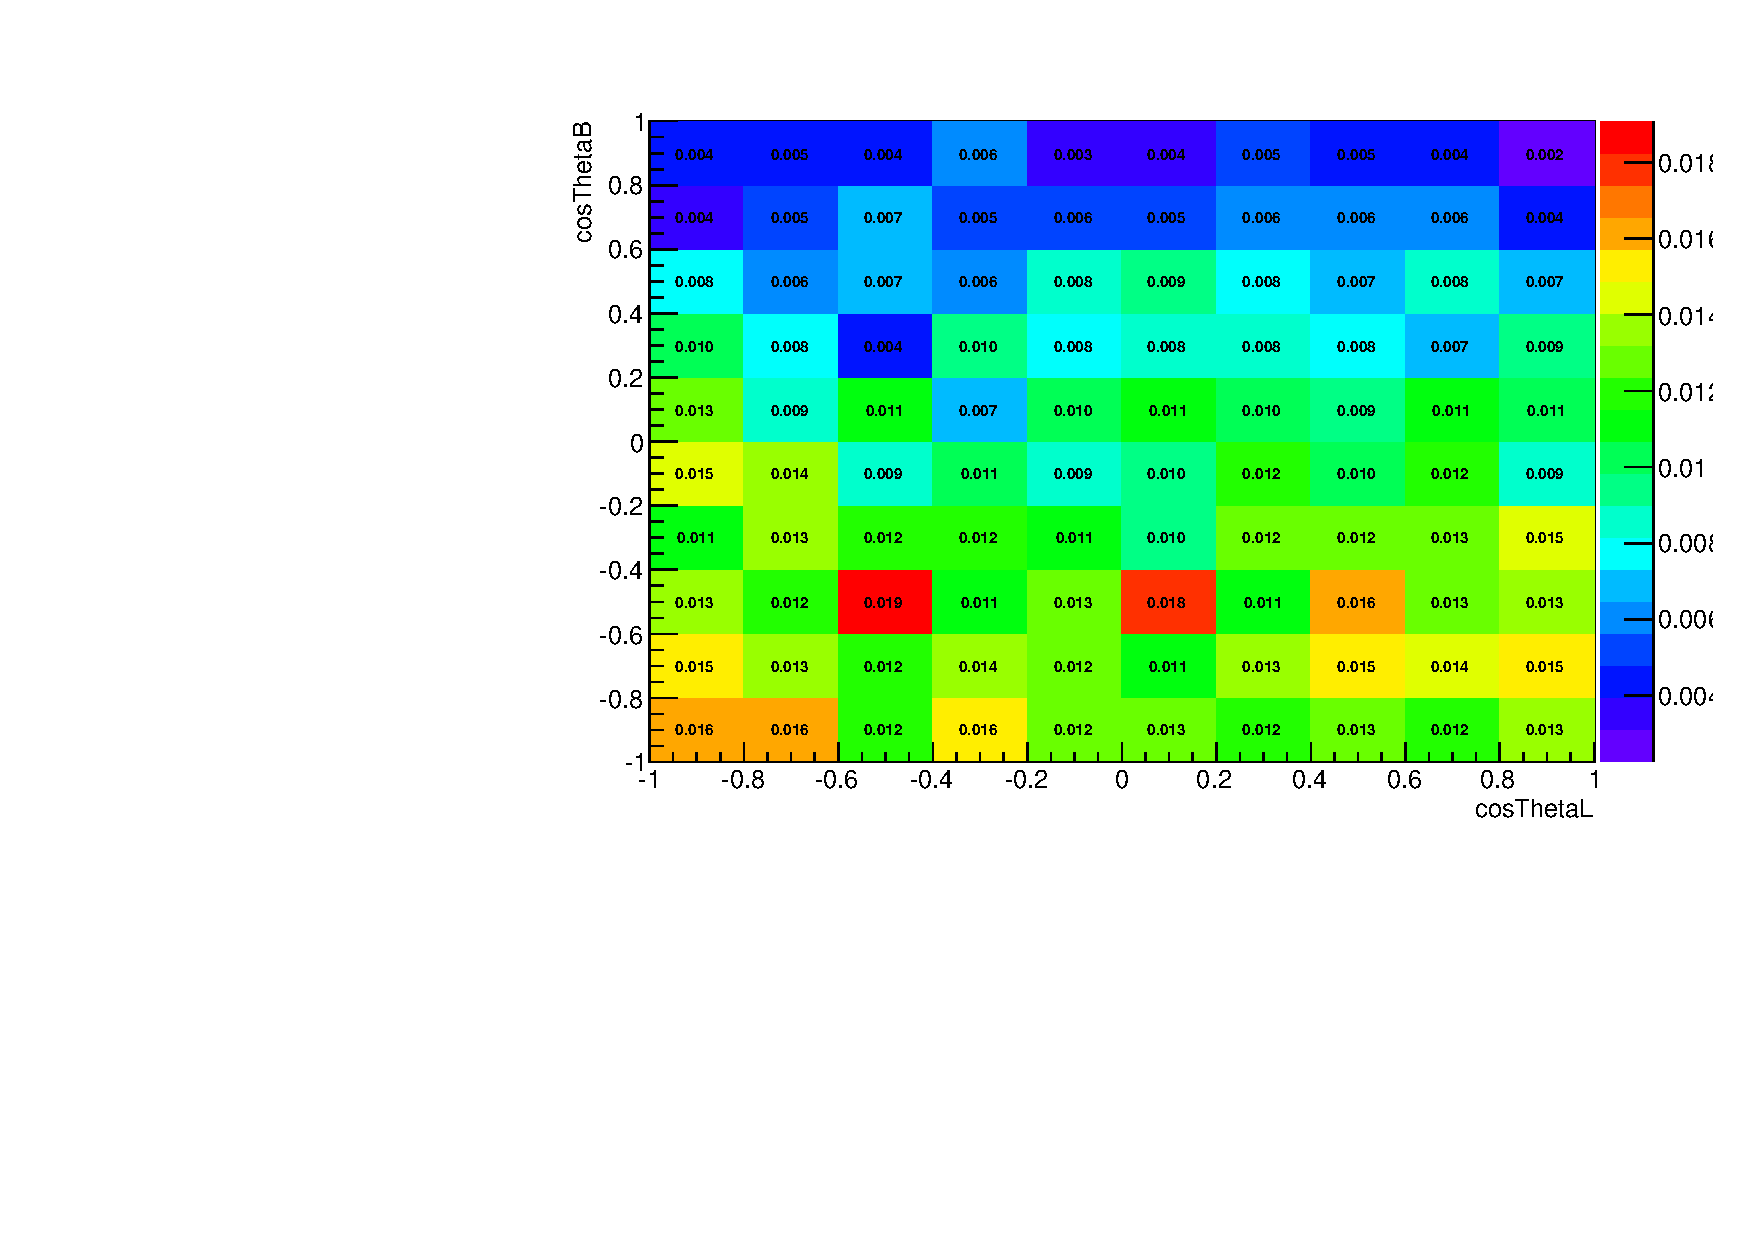
\includegraphics[width=0.9\textwidth]{Lmumu/figs/efficiencies/2D/2Deff_upper_cosThetaB_vs_cosThetaL_DD.pdf}
%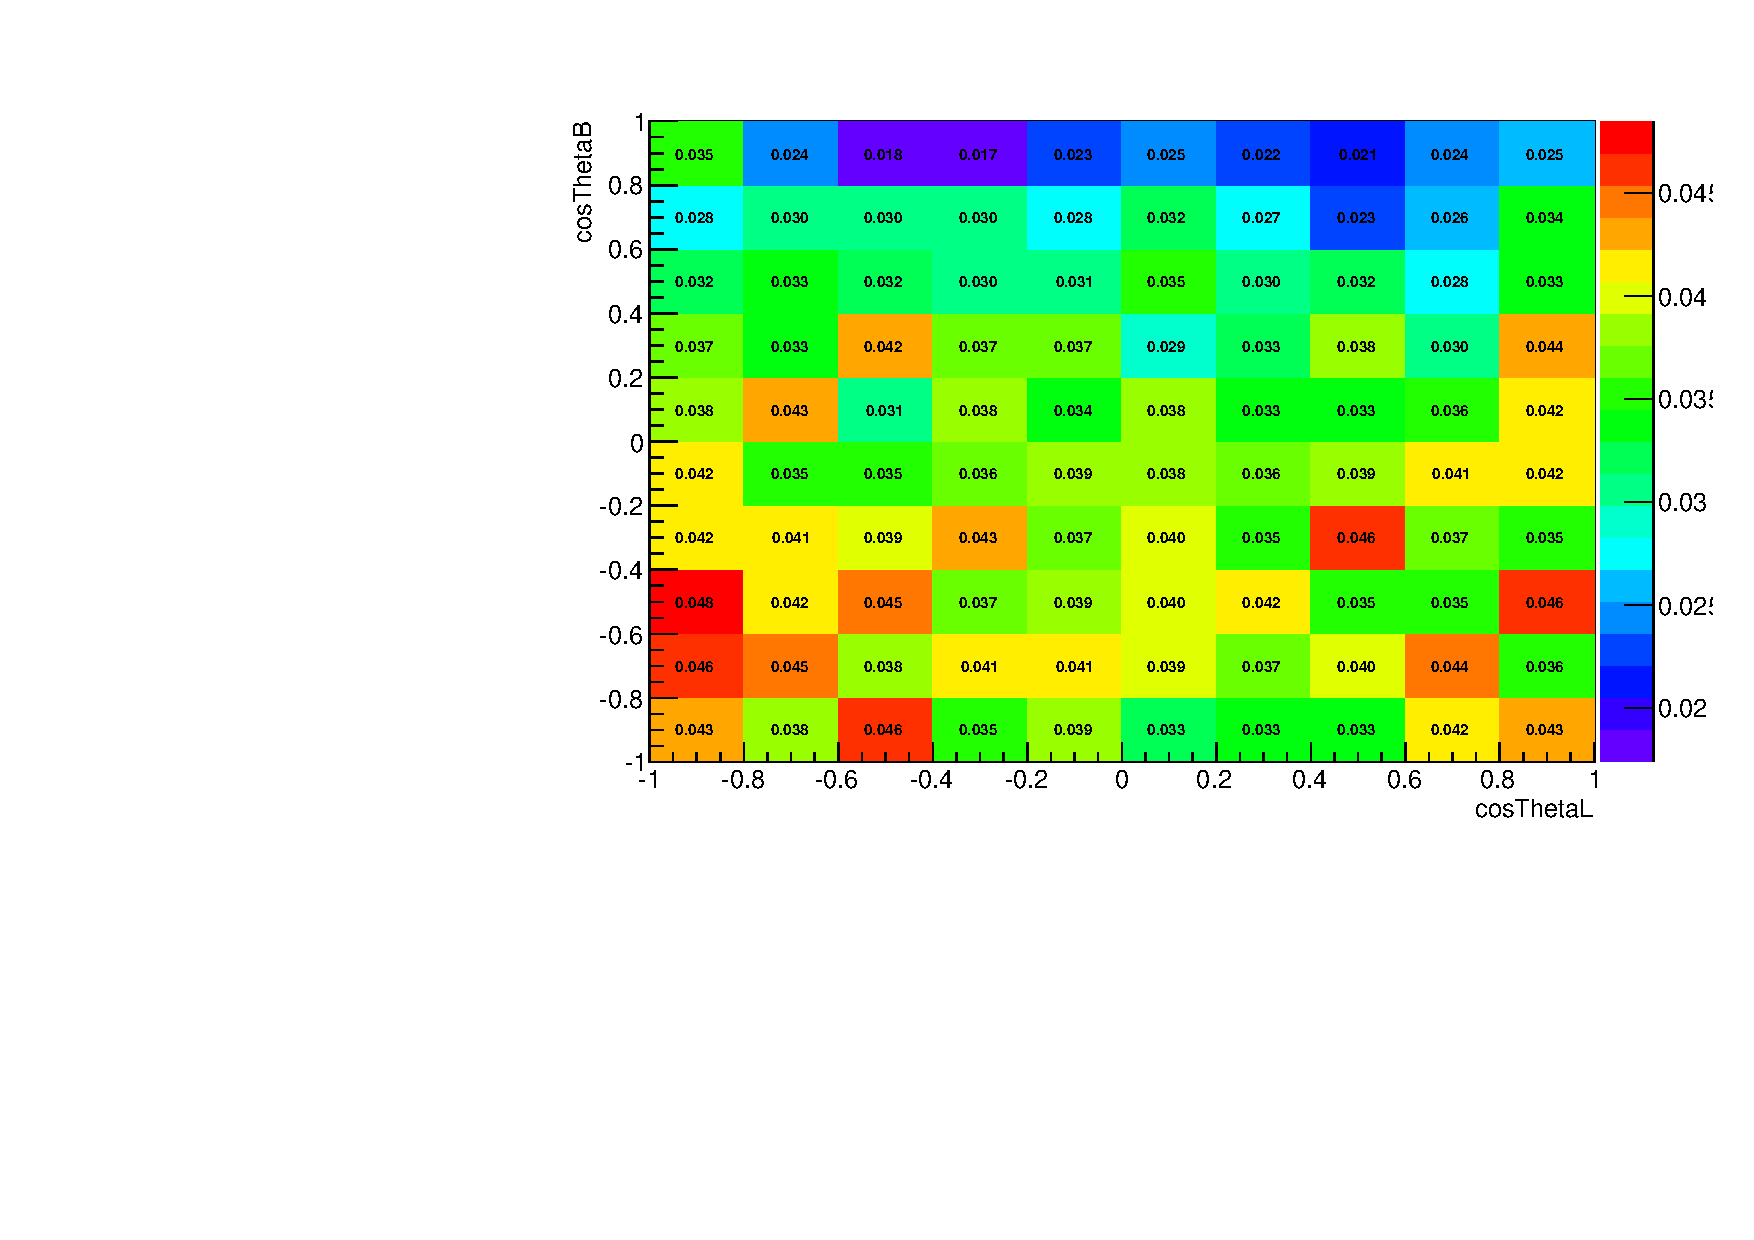
\includegraphics[width=0.9\textwidth]{Lmumu/figs/efficiencies/2D/2Deff_upper_cosThetaB_vs_cosThetaL_LL.pdf}
%\caption{Angular acceptance as a function of $\cos\theta_\ell$ and $\cos\theta_h$ for long (top) and
%downstream (bottom) candidates, integrated over the full available \qsq range.}
%\label{fig:2DcosThetaLandBeff}
%\end{figure}
%
%\begin{figure}[h!]
%\centering
%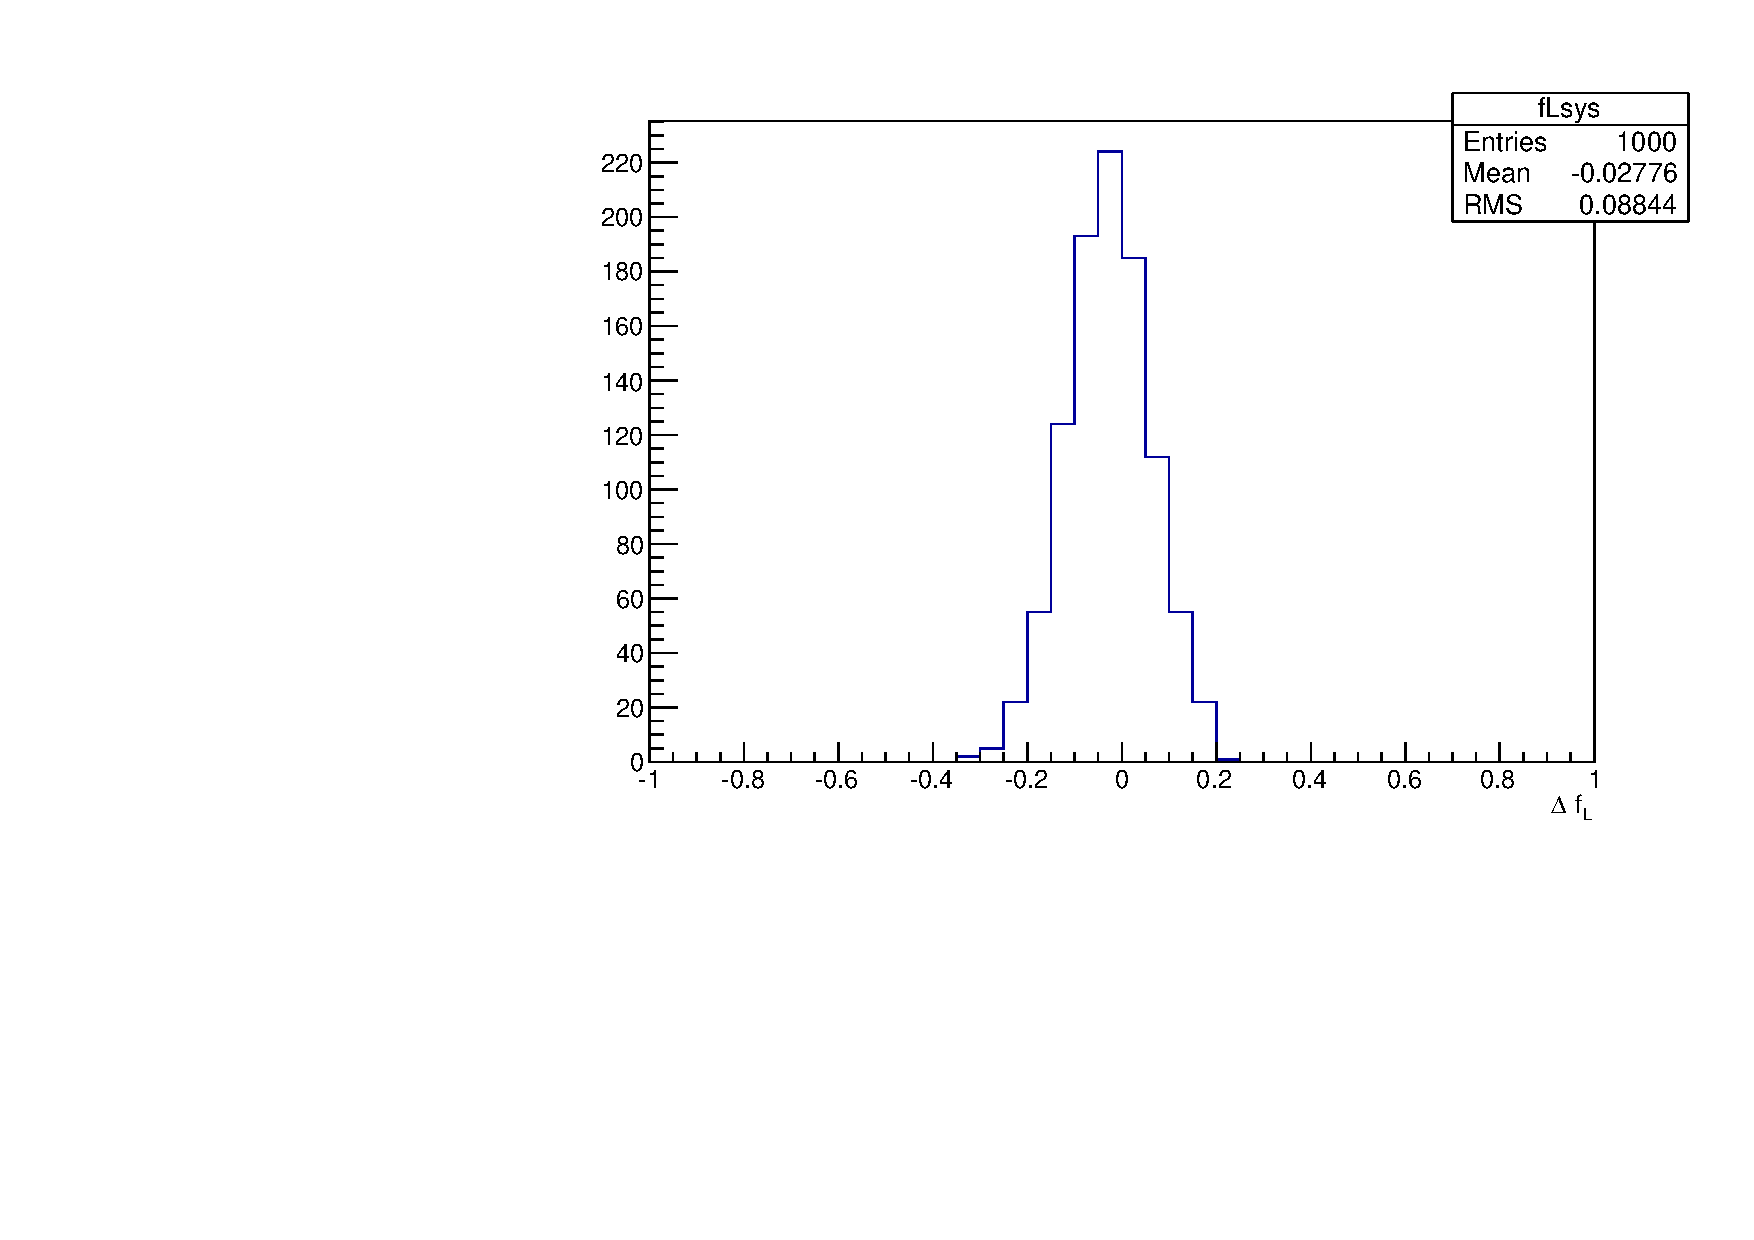
\includegraphics[width=0.49\textwidth]{Lmumu/figs/fLsys_efficiency.pdf}
%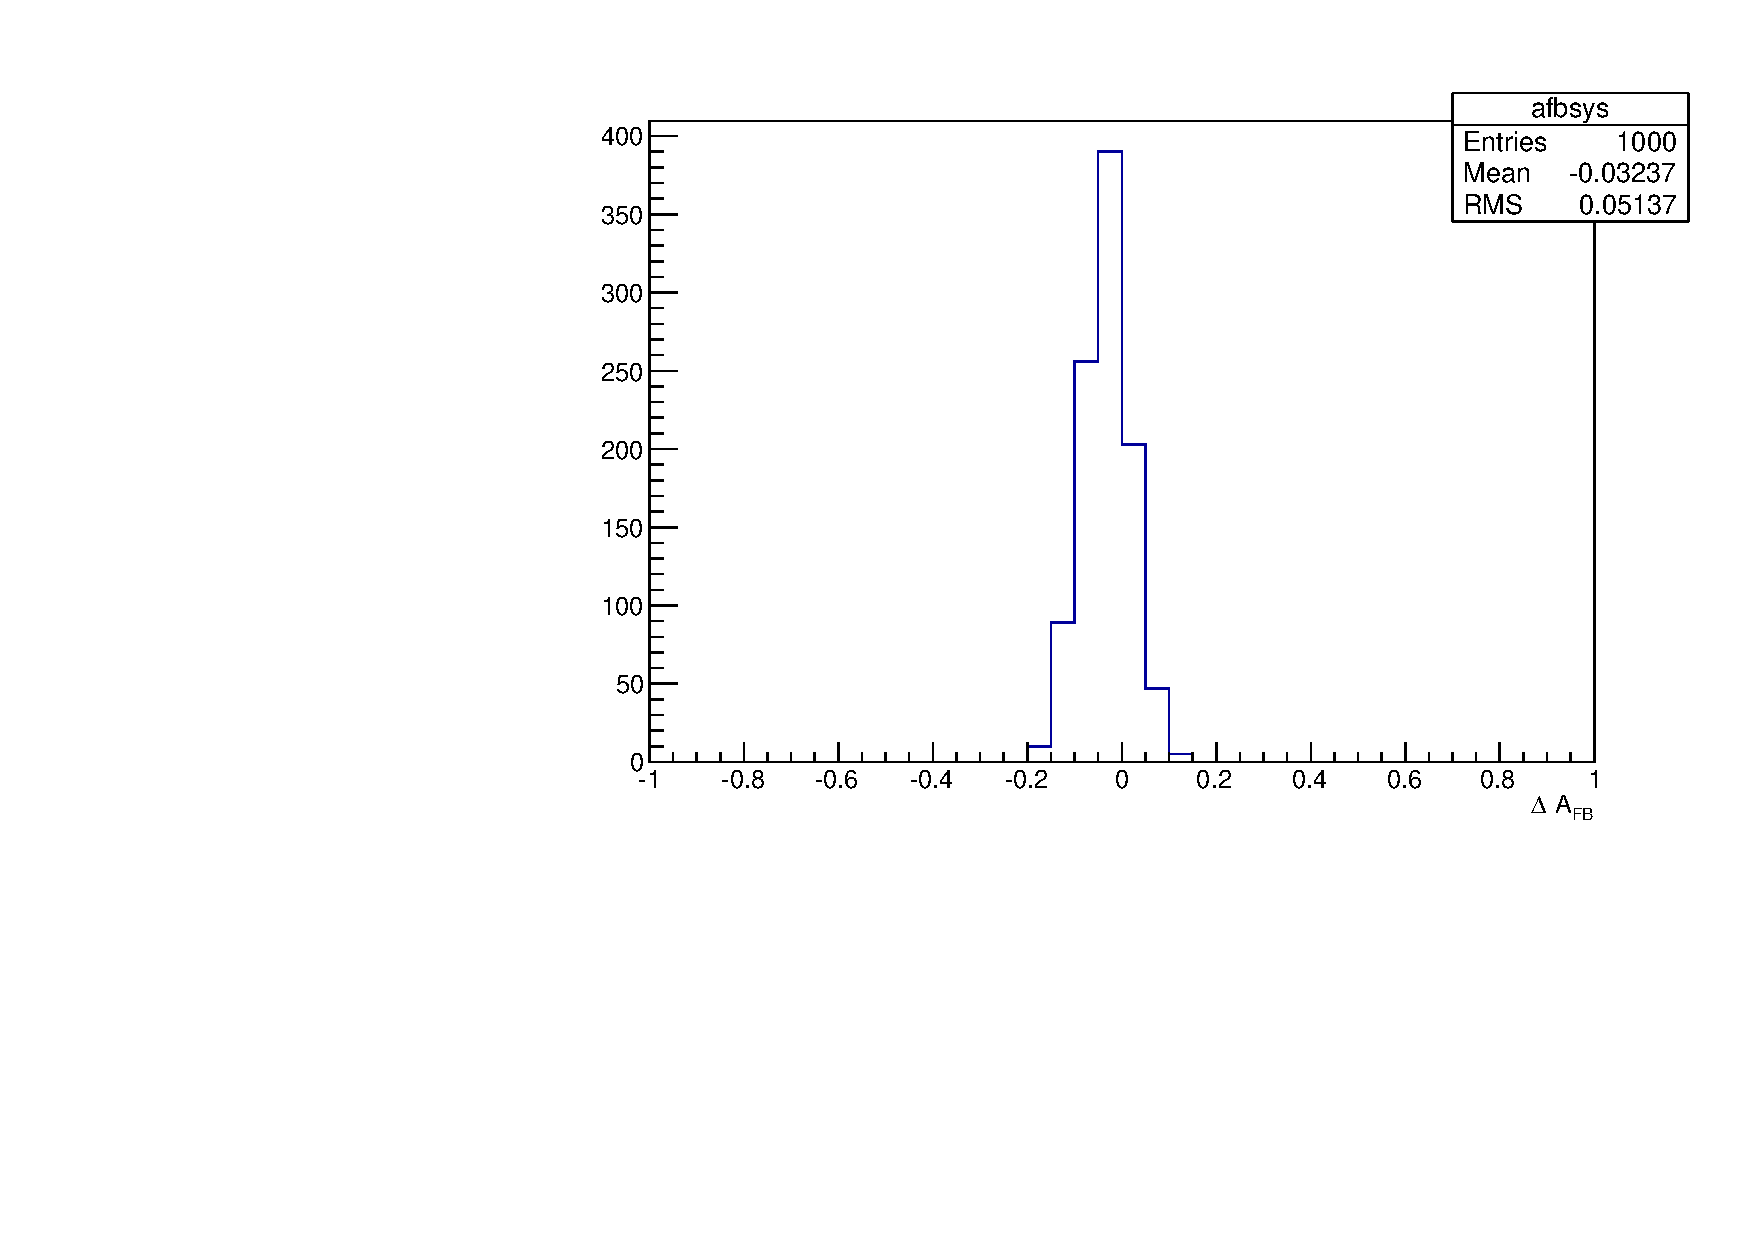
\includegraphics[width=0.49\textwidth]{Lmumu/figs/afbsys_efficiency.pdf}
%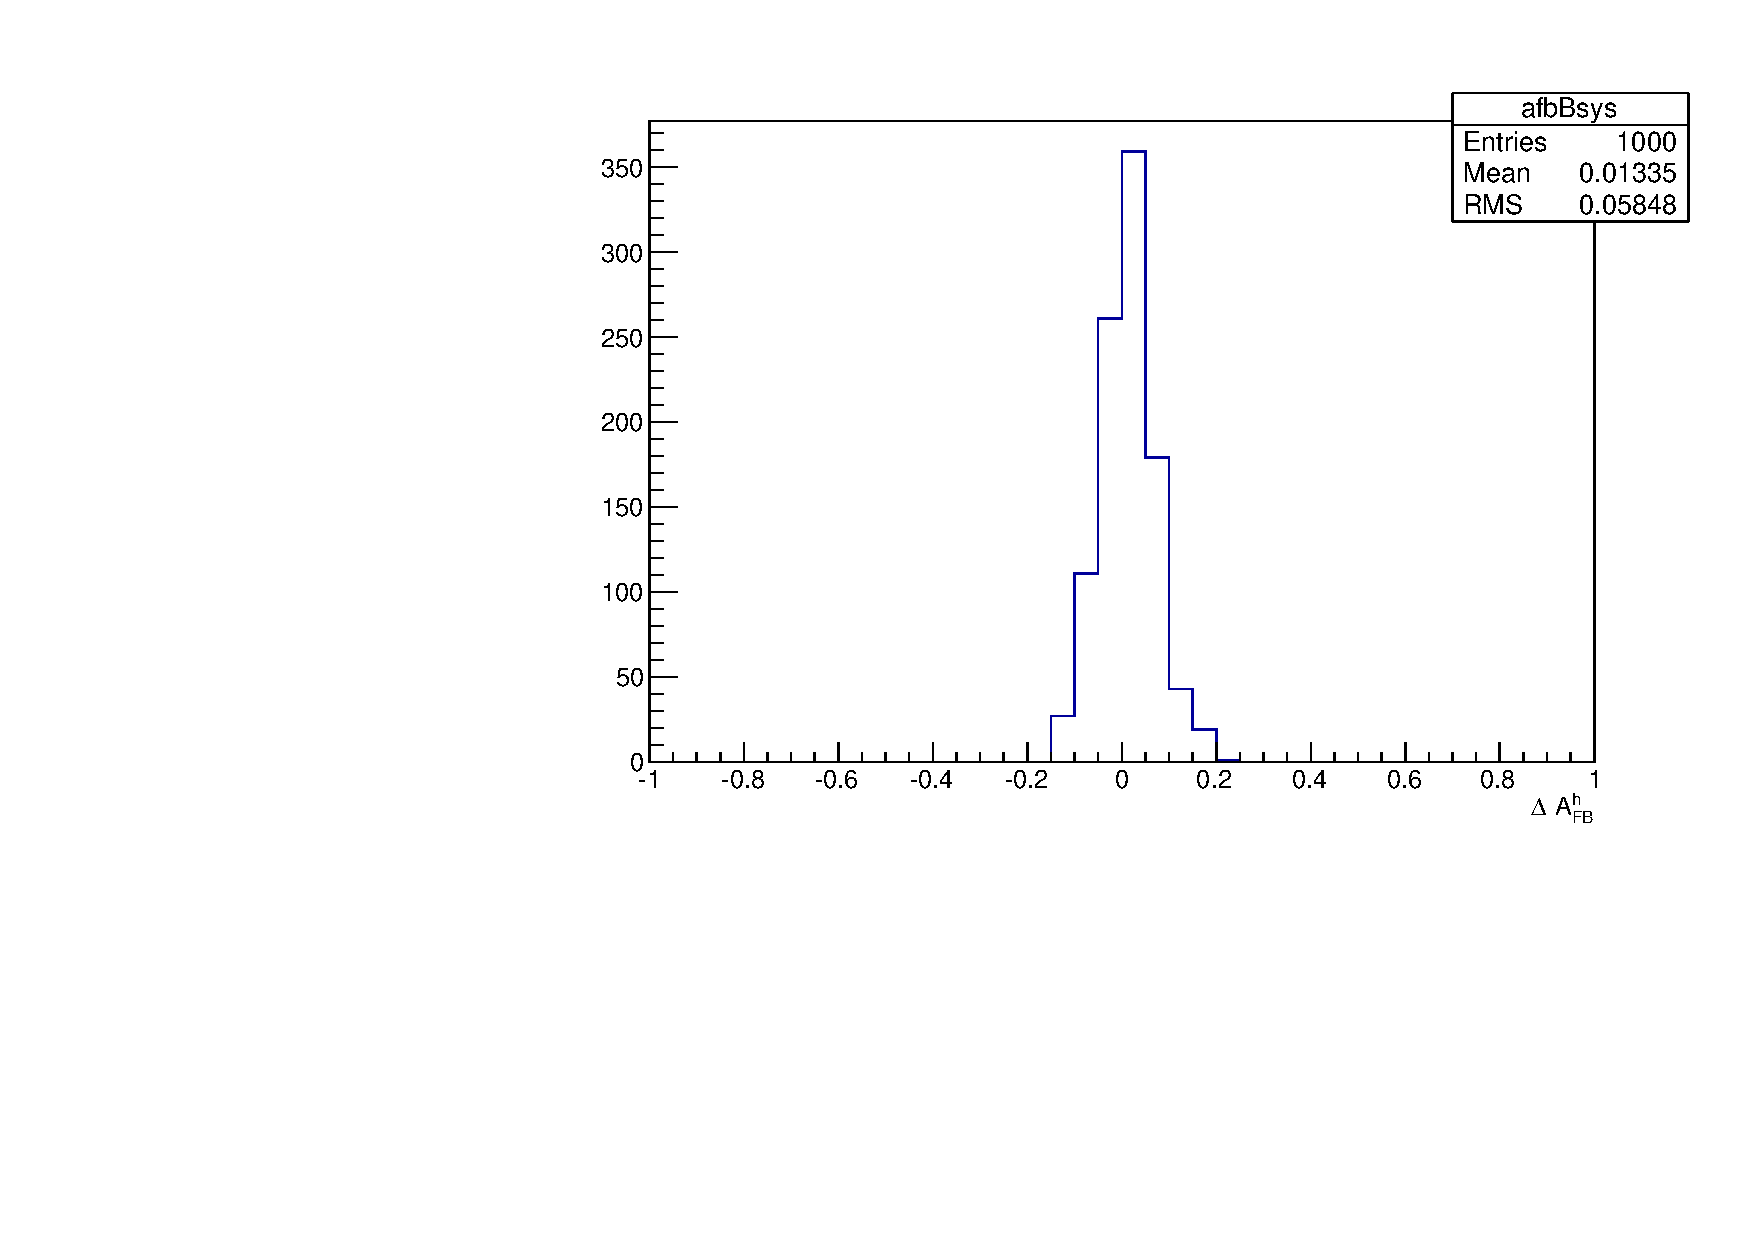
\includegraphics[width=0.49\textwidth]{Lmumu/figs/afbBsys_efficiency.pdf}
%\caption{Deviations of the observables' values obtained fitting simulated events
% generated with a 2D distribution multiplied by a 2D efficiency and fitting 1D projections
% with respect to generated values. For $\fl$ (top left), 
% $\afbl$ (top right) and $\afbh$ (bottom). }
%\label{fig:effBias}
%\end{figure}




\subsection{Resolution}

The angular resolution could bias the observables measurement 
%If the angular distribution is asymmetric, a non-zero resolution may yield to
generating an asymmetric migration of events.
This is especially important in the $\cos \theta_h$ case, due to its worse resolution
and considerably asymmetric distribution. Simulated experiments are used to asses this systematic.
Events are generated according to the measured distributions including efficiencies.
The generated events are then smeared by the angular resolution (gaussian smearing).
To be conservative the case with biggest angular resolution, downstream candidates, is always used.
%downstream events, as reported in table \ref{tab:resolutions}.
Finally, the smeared and not-smeared distributions are fit with the same PDF.  
The average deviation from the default values are reported in Tab.~\ref{tab:resolSys}
as a function of \qsq and assigned as systematic uncertainties.
%
\begin{table}[h]
\centering
\caption{Values of simulated $\cos\theta_\ell$ and $\cos\theta_\Lambda$ 
resolutions and systematic uncertainties on angular observables due to
the finite resolution in bins of \qsq.}
\begin{tabular}{c|ccccc}
 \boldmath{ \qsq [\gevgevcccc] } &  \boldmath{ $\sigma_\ell$ }    &  \boldmath{ $\sigma_\Lambda$}   & \boldmath{ $\Delta \afbl$} &  \boldmath{ $\Delta \fl$} & \boldmath{ $\Delta \afbh$ } \\ \hline
\phantom{x}0.1 -- 2.0\phantom{x}  & 0.0051 & 0.061 & 0.0011 & -0.0022 & -0.007 \\ 
11.0 -- 12.5 & 0.0055 & 0.067 & 0.0016 & -0.0051 & -0.013 \\
15.0 -- 16.0 & 0.0059 & 0.070 & 0.0006 & -0.0054 & -0.010 \\
16.0 -- 18.0 & 0.0064 & 0.070 & 0.0014 & -0.0077 & -0.010 \\
18.0 -- 20.0 & 0.0081 & 0.074 & 0.0014 & -0.0062 & -0.010 \\
\hline
15.0 -- 20.0 & 0.0066 & 0.072 & 0.0013 & -0.0076 & -0.011 \\
\end{tabular}
\label{tab:resolSys}
\end{table}


\subsection{Efficiency description}

An imprecise determination of the reconstruction and selection efficiency can introduce an extra oddity
and therefore bias the measurement. To asses this effect the kinematic re-weighting described in Sec.~\ref{sec:kinWeight}
is removed from the simulation and the efficiency is determined again.
Simulated events are then fit using the same theoretical PDF and multiplied by the efficiency
functions obtained with and without kinematical weights. As in the previous cases the average bias 
is taken as systematic uncertainty; results are shown in Tab.~\ref{tab:AfbeffSys}.
Furthermore, the effect of the limited simulated statistics is taken into account and 
added to the systematic uncertainty.
%This is not already taken in account
%by the Feldman-Cousins plug-in method ( see \ref{sec:FeldmanCousins}) since the efficiency parameters are always fixed
%in the fit. We generate toy MC events using the measured values of angular observables and the default efficiency. 
%Then we vary the efficiency with its errors and we refit with the new efficiency model. In each toy we generate a number
%of events comparable to the one we have in data in bins of \qsq. The average deviation over 1000 toys is taken as systematic,
%values are reported in table \ref{tab:stateffsys}. N.B.: Efficiency parameters are always fixed when fitting the angular distributions. 
%
%Finally, the effect induced by a non-zero production polarisation in the efficiency description
%was investigated by varying the polarisation parameter in the model used to re-weight the simulation
%from $- \sigma$ to $+ \sigma$ for the central measured value, as done for the branching ratio analysis \ref{sec:BRpolsys}. 
%Then again simulated experiments are generated and fit using efficiency models obtained with different values
%of the polarisation. No significant effect is found. 
%
\begin{table}[h]
\centering
\caption{Values systematic uncertainties due to limited knowledge of the efficiency
function on the three angular observables in bins of \qsq}
\begin{tabular}{c|ccc}
 \boldmath{ \qsq [\gevgevcccc] }  &  \boldmath{ \afbl }   &  \boldmath{ \fl} &  \boldmath{ \afbh} \\ \hline
\phantom{x}0.1 -- 2.0\phantom{x}    	 & 0.0020  & 0.0440 &  0.0093\\ 
11.0 -- 12.5  					 & 0.0069  & 0.0027 &  0.0069\\
15.0 -- 16.0  					 & 0.0018  & 0.0046 &  0.0109\\
16.0 -- 18.0  					 & 0.0012  & 0.0043 &  0.0159\\
18.0 -- 20.0  					 & 0.0030  & 0.0017 &  0.0148\\
\hline
15.0 -- 20.0  					 & 0.0002  & 0.0046 &  0.0138\\
\end{tabular}
\label{tab:AfbeffSys}
\end{table}
\begin{table}[h]
\centering
\caption{Values of systematic uncertainties due to the statistics of the simulated
samples on the three angular observables in bins of \qsq.}
\begin{tabular}{c|ccc}
\boldmath{ \qsq [\gevgevcccc] } &  \boldmath{ $\afbl$}   &  \boldmath{ \fl } &  \boldmath{ $\afbh$ } \\ \hline
\phantom{x}0.1 -- 2.0\phantom{x}     &  0.00151 & 0.00170  & 0.00213 \\
11.0 -- 12.5  &  0.00121 & 0.00154  & 0.00196 \\
15.0 -- 16.0  &  0.00004 & 0.00017  & 0.00103 \\
16.0 -- 18.0  &  0.00065 & 0.00246  & 0.00417 \\
18.0 -- 20.0  &  0.00023 & 0.00372  & 0.00162 \\
\hline
15.0 -- 20.0  &  0.00039 & 0.00091  & 0.00137 \\
\end{tabular}
\label{tab:stateffsys}
\end{table}


\subsection{Background parameterisation}
\label{sec:bkgShapeSys}

There is a certain degree of arbitrariety in the choice of a parameterisation for the background,
especially for \qsq intervals with low statistics. To asses possible biases due to the choice of a specific PDF, simulated experiments
are generated using the shapes obtained from fits to data and the same statistics as observed in data for each \qsq interval.
Each pseudo-experiment is fit with two models: the default one, a ``line times efficiency" function and
the efficiency function alone, corresponding to the assumption that background distributions
are originally flat and only modified by the interaction with the detector. 
The average bias with respect to the default model is taken as systematic uncertainty;
results are reported in Tab.~\ref{tab:bkgParamSys}.
%
%Finally, we consider also the bias which may be cause by fixing the background fraction in the fit by fitting the same toys with
%a model where the background fraction is fixed to a random value normally distributed around the measured one. This systematic is negligible
%compared to the previous one but we add it anyway to the final systematic.
%The total result calculated as the square root sum of the 2 compoents is reported in table \ref{tab:bkgParamSys}.
%
\begin{center}
\begin{table}[h]
\centering
\caption{ Values of systematic uncertainties due to the choice of background parameterisation in bins of \qsq. }
\begin{tabular}{c|ccc}
 \boldmath{ \qsq [\gevgevcccc] } &  \boldmath{ $\afbl$ }     &  \boldmath{  $\fl$ }      &  \boldmath{ $\afbh$   } \\ \hline
\phantom{x}0.1 -- 2.0\phantom{x}         &  0.003	 &   0.049	  &  0.053		\\
11.0 -- 12.5		&  0.045     &   0.034	  &  0.035     \\
15.0 -- 16.0 	&  0.010     &   0.038    &  0.026     \\
16.0 -- 18.0 	&  0.026     &   0.036    &  0.022     \\
18.0 -- 20.0 	&  0.011     &   0.031    &  0.025     \\
\hline
15.0 -- 20.0		&  0.007     &   0.014    &  0.017     \\
\end{tabular}
\label{tab:bkgParamSys}
\end{table}
\end{center}




\subsection{Polarisation}
\label{sec:ang_pol_sys}

To study the effect of a non-zero \Lb production polarisation simulated events are generated 
using the distributions given by Eqs.~\ref{eq:lepton2D} and~\ref{eq:hadron2D} as a function of the
angle under study ($\cos\theta_\ell$ or $\cos\theta_h$) and $\cos\theta$, defined in Sec.~\ref{sec:multidim_ang_distrib}, 
which is sensitive to polarisation.
Similarly to the procedure used for the branching ratio measurement, events are generated varying
the value of the polarisation within one standard deviation from the LHCb measurement~\cite{Aaij:2013oxa}.
As in the theoretical functions $\cos \theta$ is always odd, it would always
drop out when integrating over $\theta$ in the case of perfect efficiency, yielding no bias by contruction. Therefore, the 
generated distributions are also multiplied by the two-dimensional efficiency function. No significant bias is found.
%In Fig.~\ref{fig:2Deffs} are reported 2D efficiencies
%as a function of $\cos \theta_\ell$ and $\cos \theta_\Lambda$ versus $\cos \theta$. and in Fig.~\ref{fig:Afbpolsys} are reported distributions of the absolute difference between the observable value obtained fitting generated events with the two polarisation values. 
%We then plot the the biggest difference between the plus or minus $\sigma$ case and the central value.
%For the integrated high \qsq region we obtain the following average deviations: $\Delta \fl = 0.0016 \pm 0.0012$, $\Delta \afbl = 0.00048 \pm 0.00074$ and $\Delta \afbh = 0.00014 \pm 0.00075$.
%Since all average differences are consistent with zero within less than 1.5$\sigma$ we do not assign extra systematics for polarisation.

%\begin{figure}
%\centering
%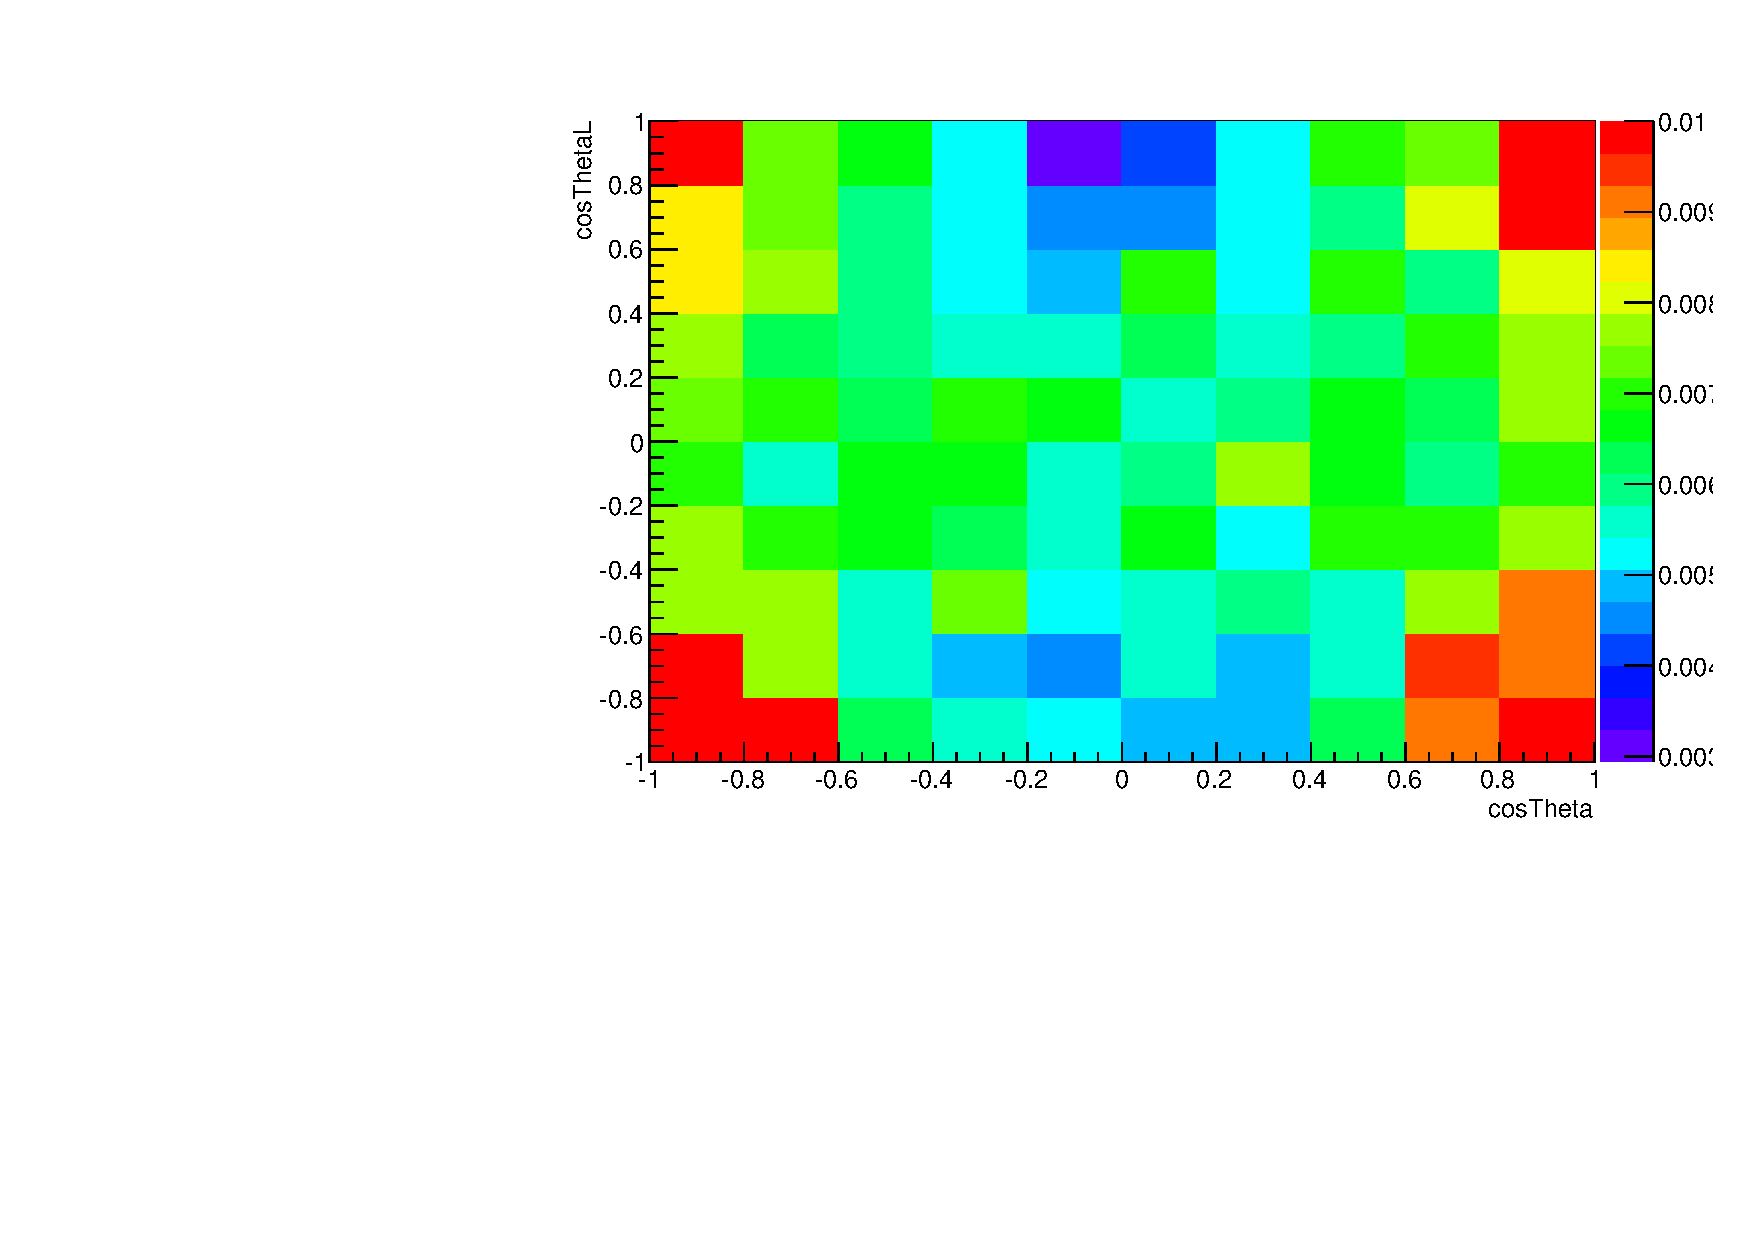
\includegraphics[width=0.45\textwidth]{Lmumu/figs/2Deff_tot_cosThetaL_vs_cosTheta_All.pdf}
%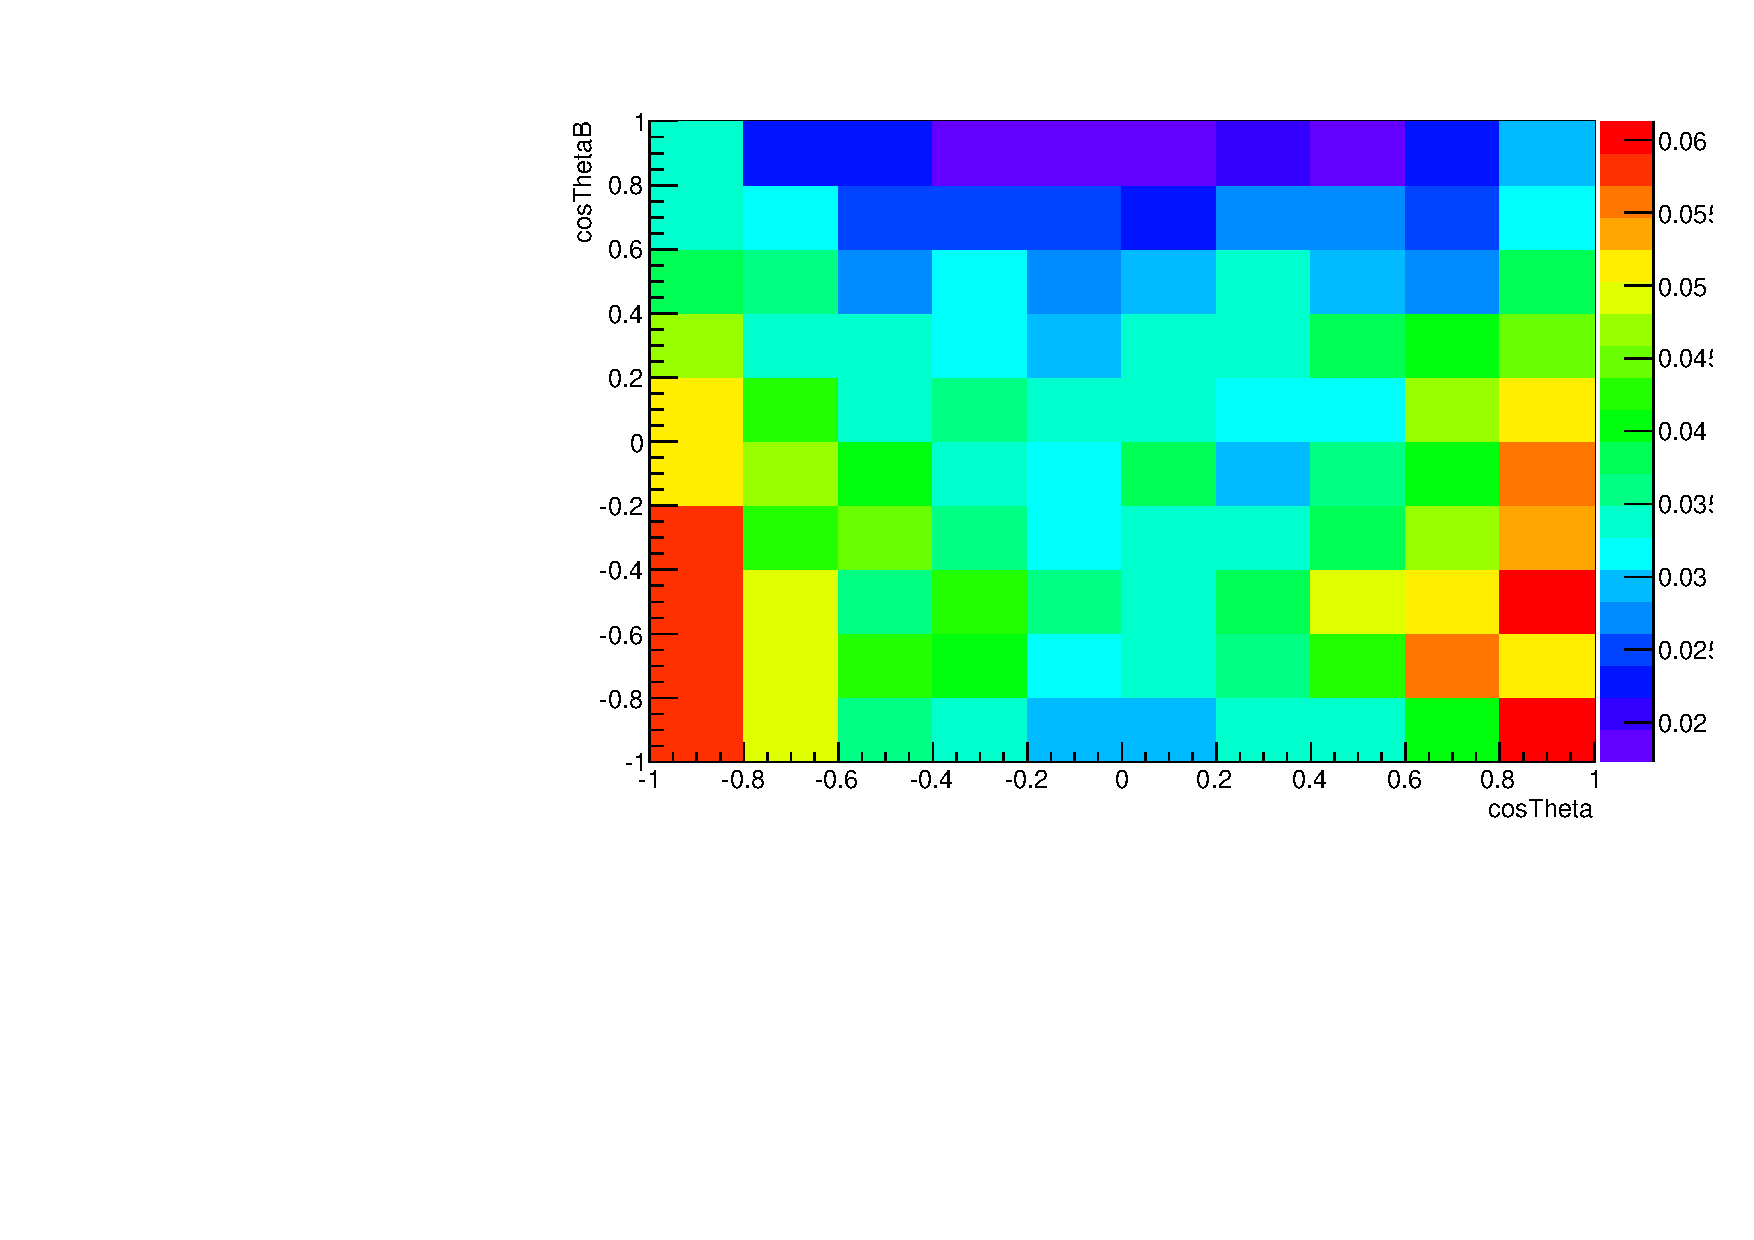
\includegraphics[width=0.45\textwidth]{Lmumu/figs/2Deff_upper_cosThetaB_vs_cosTheta_All.pdf}
%\caption{2-dimensional efficiencies obtained from weighted MC for $\cos \theta_\ell$ and $\cos\theta_\Lambda$ versus $\cos\theta$.}
%\label{fig:2Deffs}
%\end{figure}
%\begin{figure}
%\centering
%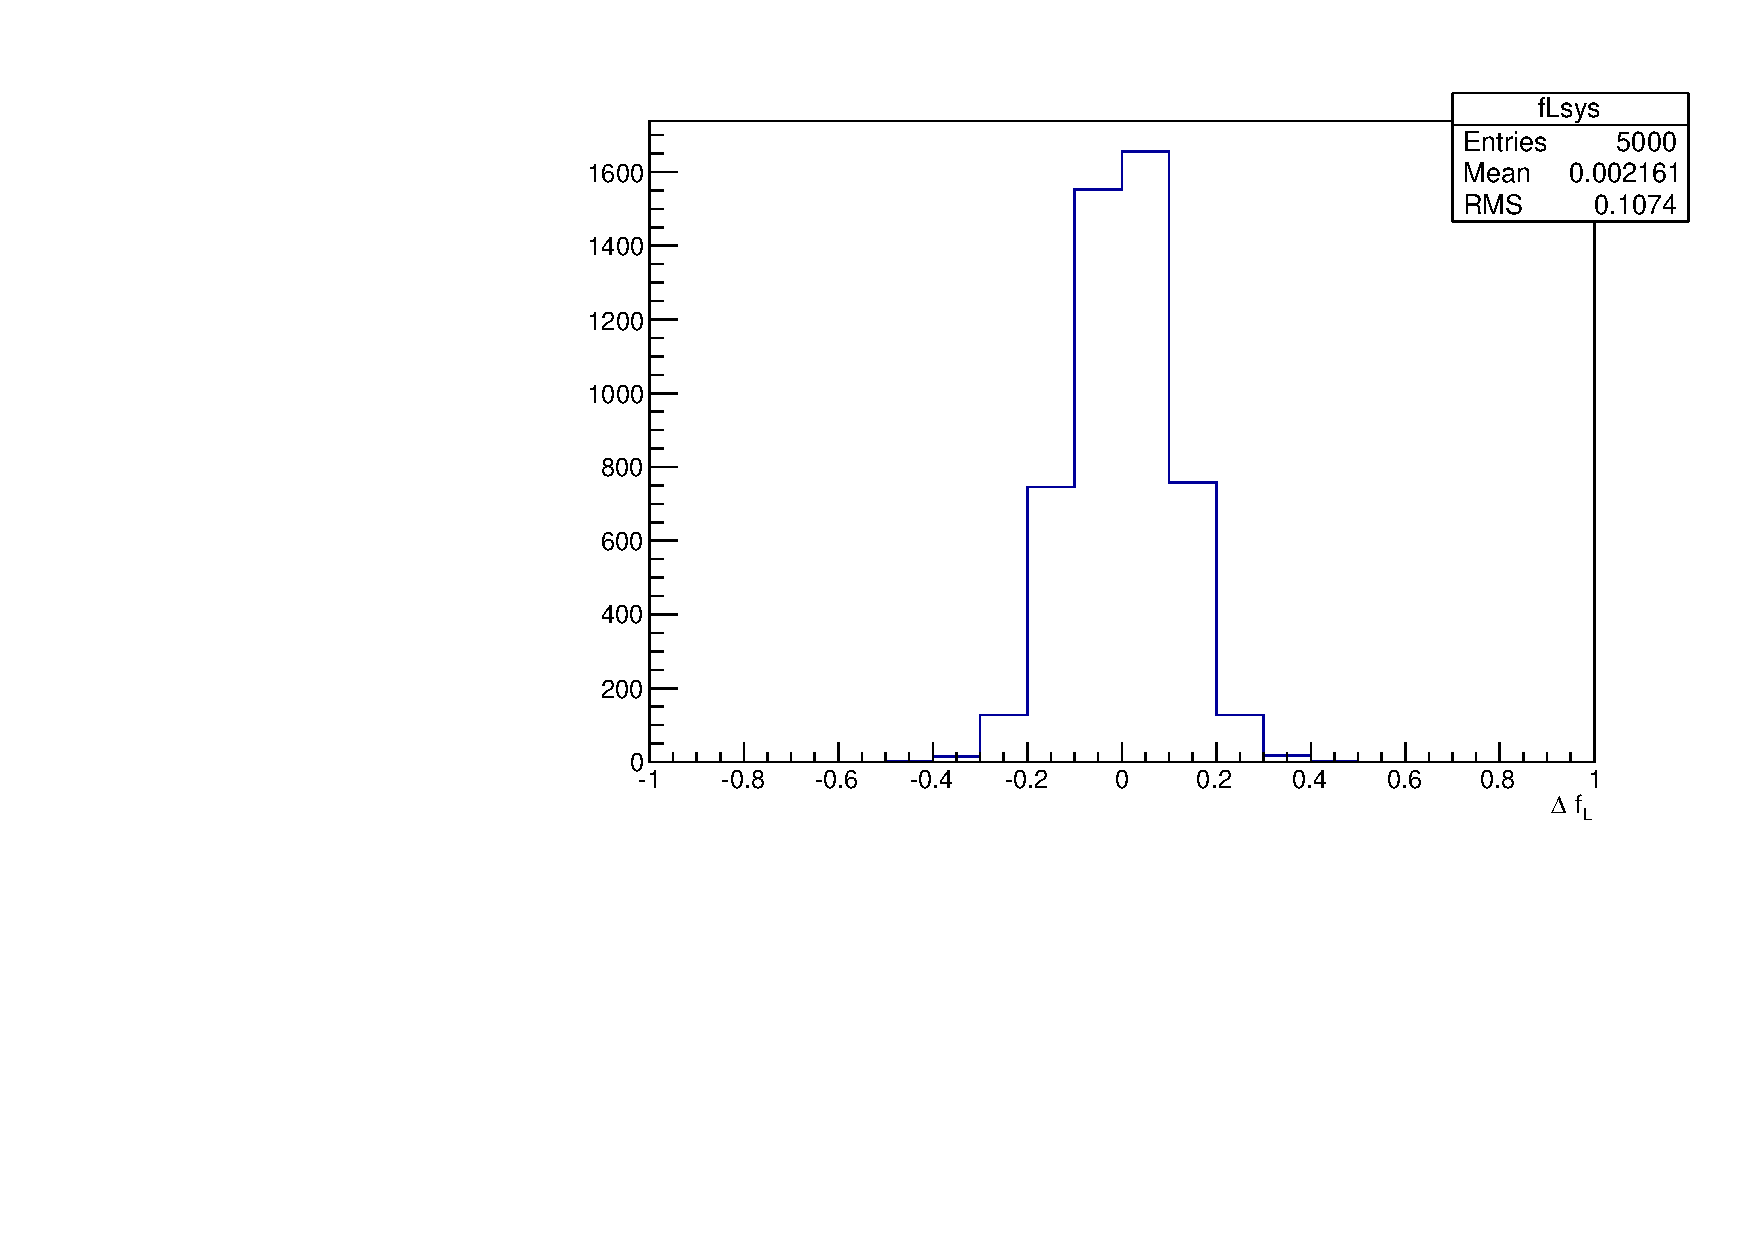
\includegraphics[width=0.45\textwidth]{Lmumu/figs/fLsys_polarisation.pdf}
%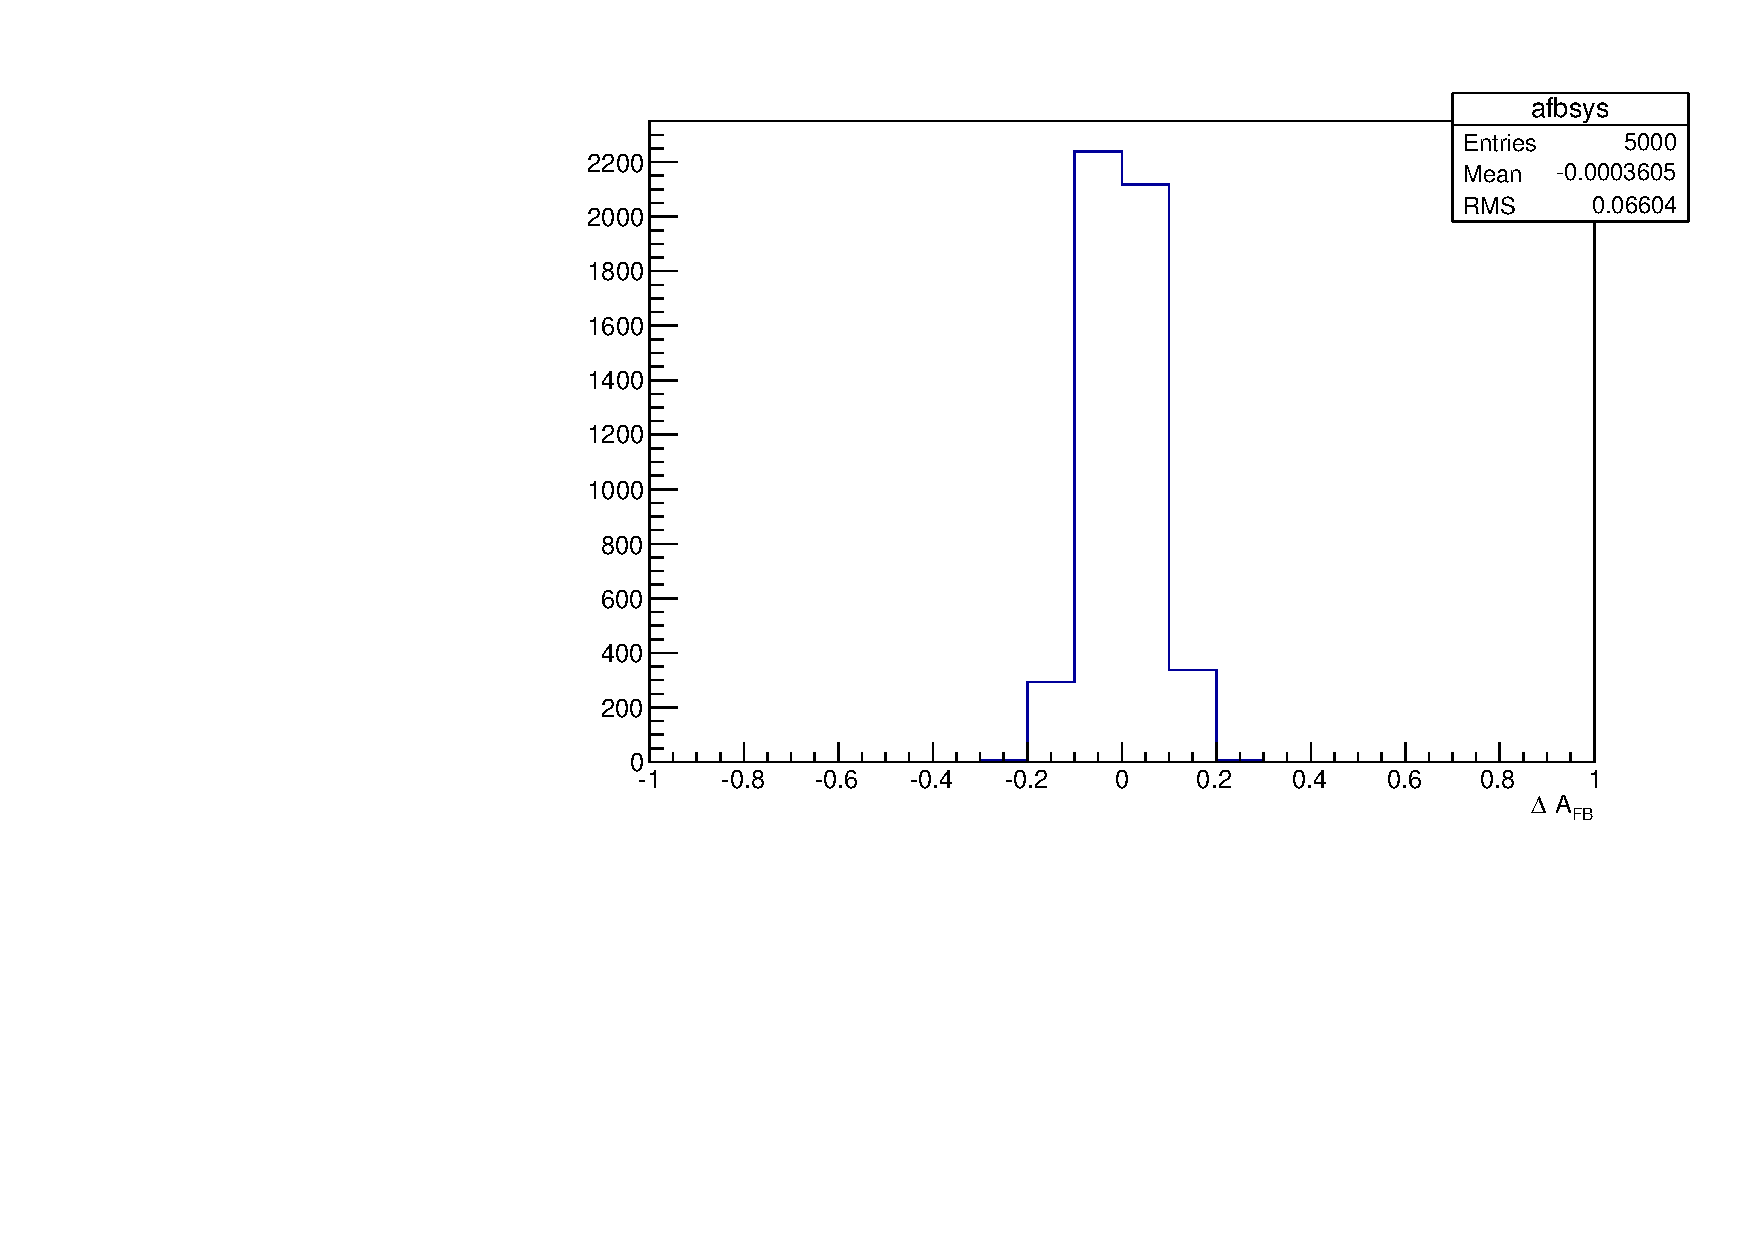
\includegraphics[width=0.45\textwidth]{Lmumu/figs/afbsys_polarisation.pdf}
%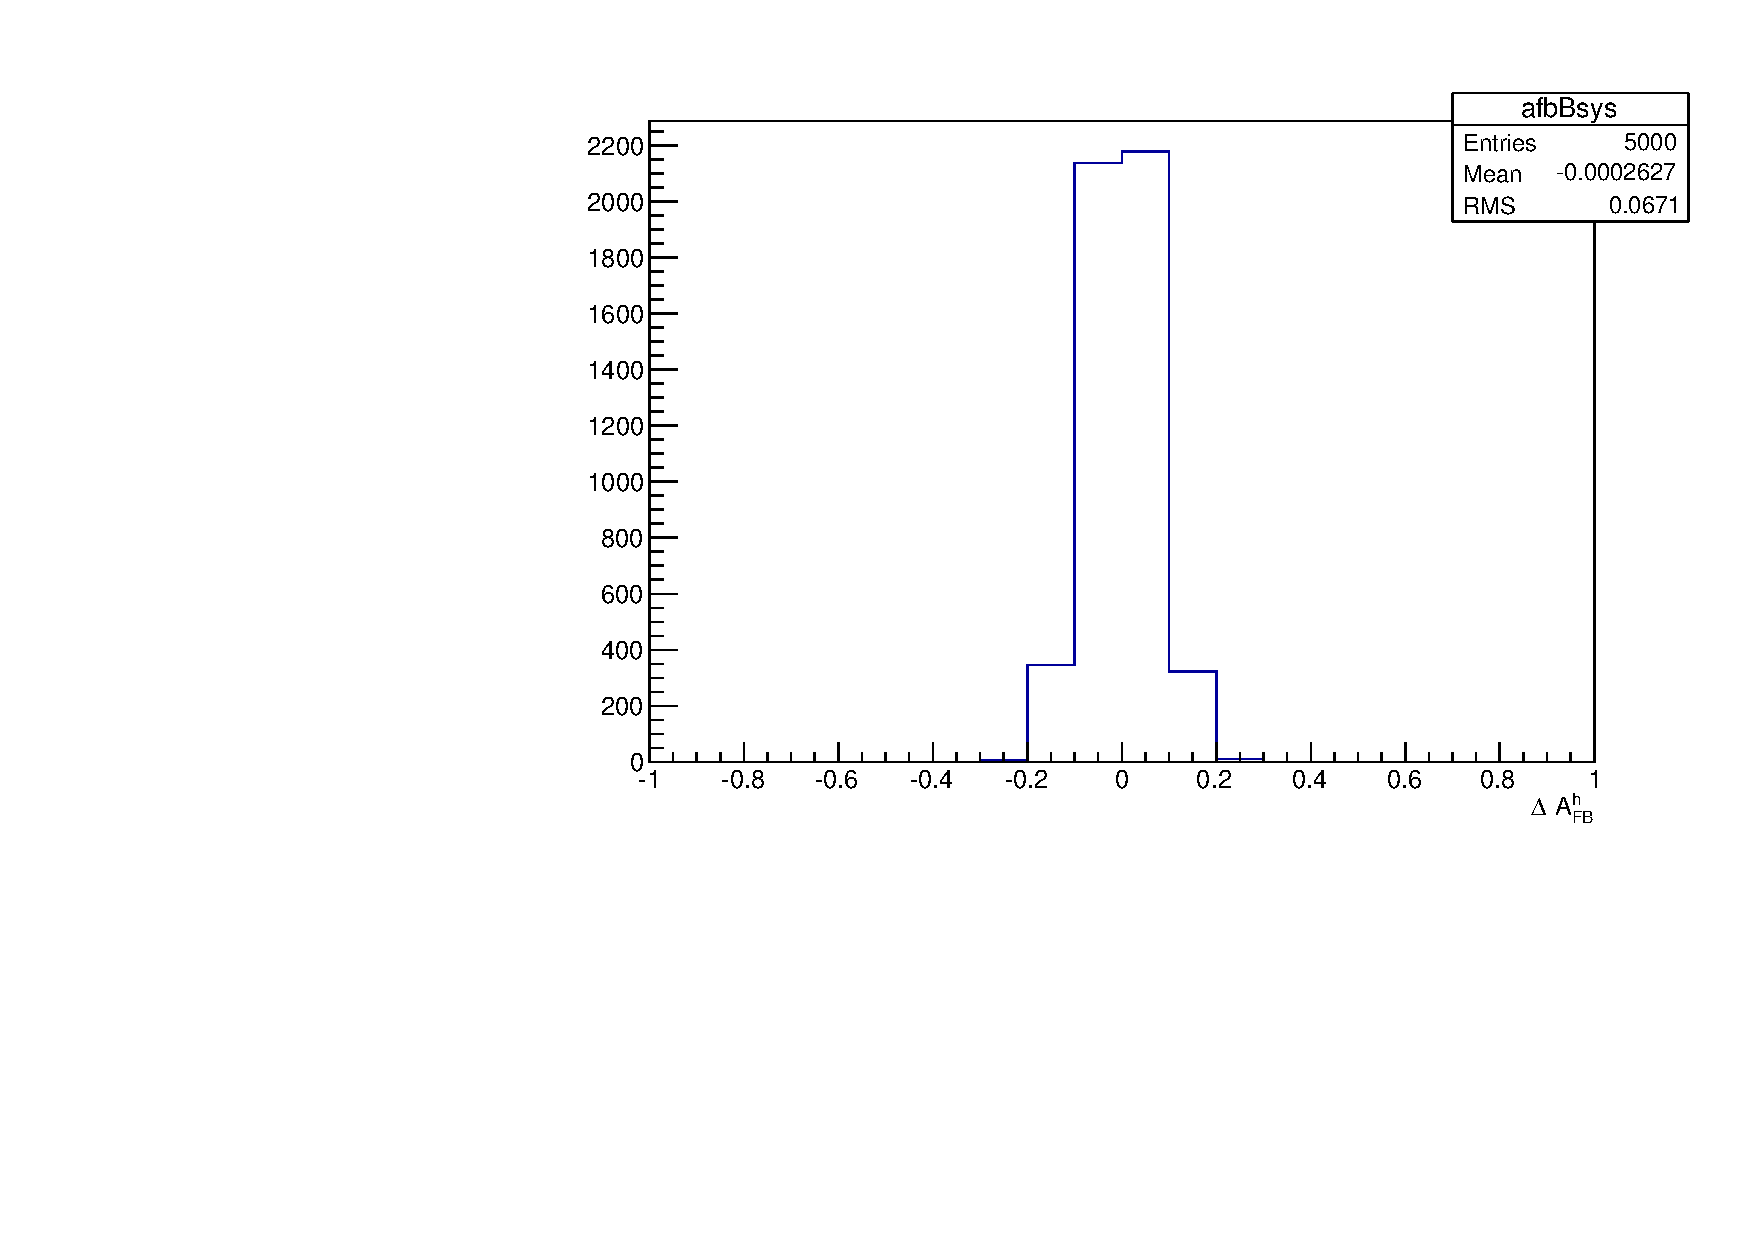
\includegraphics[width=0.45\textwidth]{Lmumu/figs/afbBsys_polarisation.pdf}
%\caption{Plots show the absolute difference of the observables' values obtained fitting toy MC generated with polarisation set to $-0.03$ and $+0.15$. From left to right for $\fl$, $\afbl$ and $\afbh$. }
%\label{fig:Afbpolsys}
%\end{figure}




\section{$J/\psi$ cross-check}

To validate the fitting procedure this is applied to the high statistics $\Lb\to\jpsi\Lz$ sample.
For this purpose events are selected with an additional requirement on the proton PID, \verb!PID!p$ > 10$.
This is needed to reduce the $\Bz\to\KS\jpsi$ background, which is particularly important for the hadronic side fit, 
since the \KS events are not distributed in a flat way in the $\cos\theta_h$ variable and would therefore bias the fit.
Figure~\ref{fig:Jpsimass_angular} shows the invariant mass distributions after this requirement is applies, which 
can be compared with the ones in Fig.~\ref{fig:Lb_totalFit}. %One can see that the \KS background is reduced.
After the PID cut there are 0.2\% of \KS events left in the downstream sample and a fraction
compatible with zero in the long sample.
%
\begin{figure}[b]
\centering
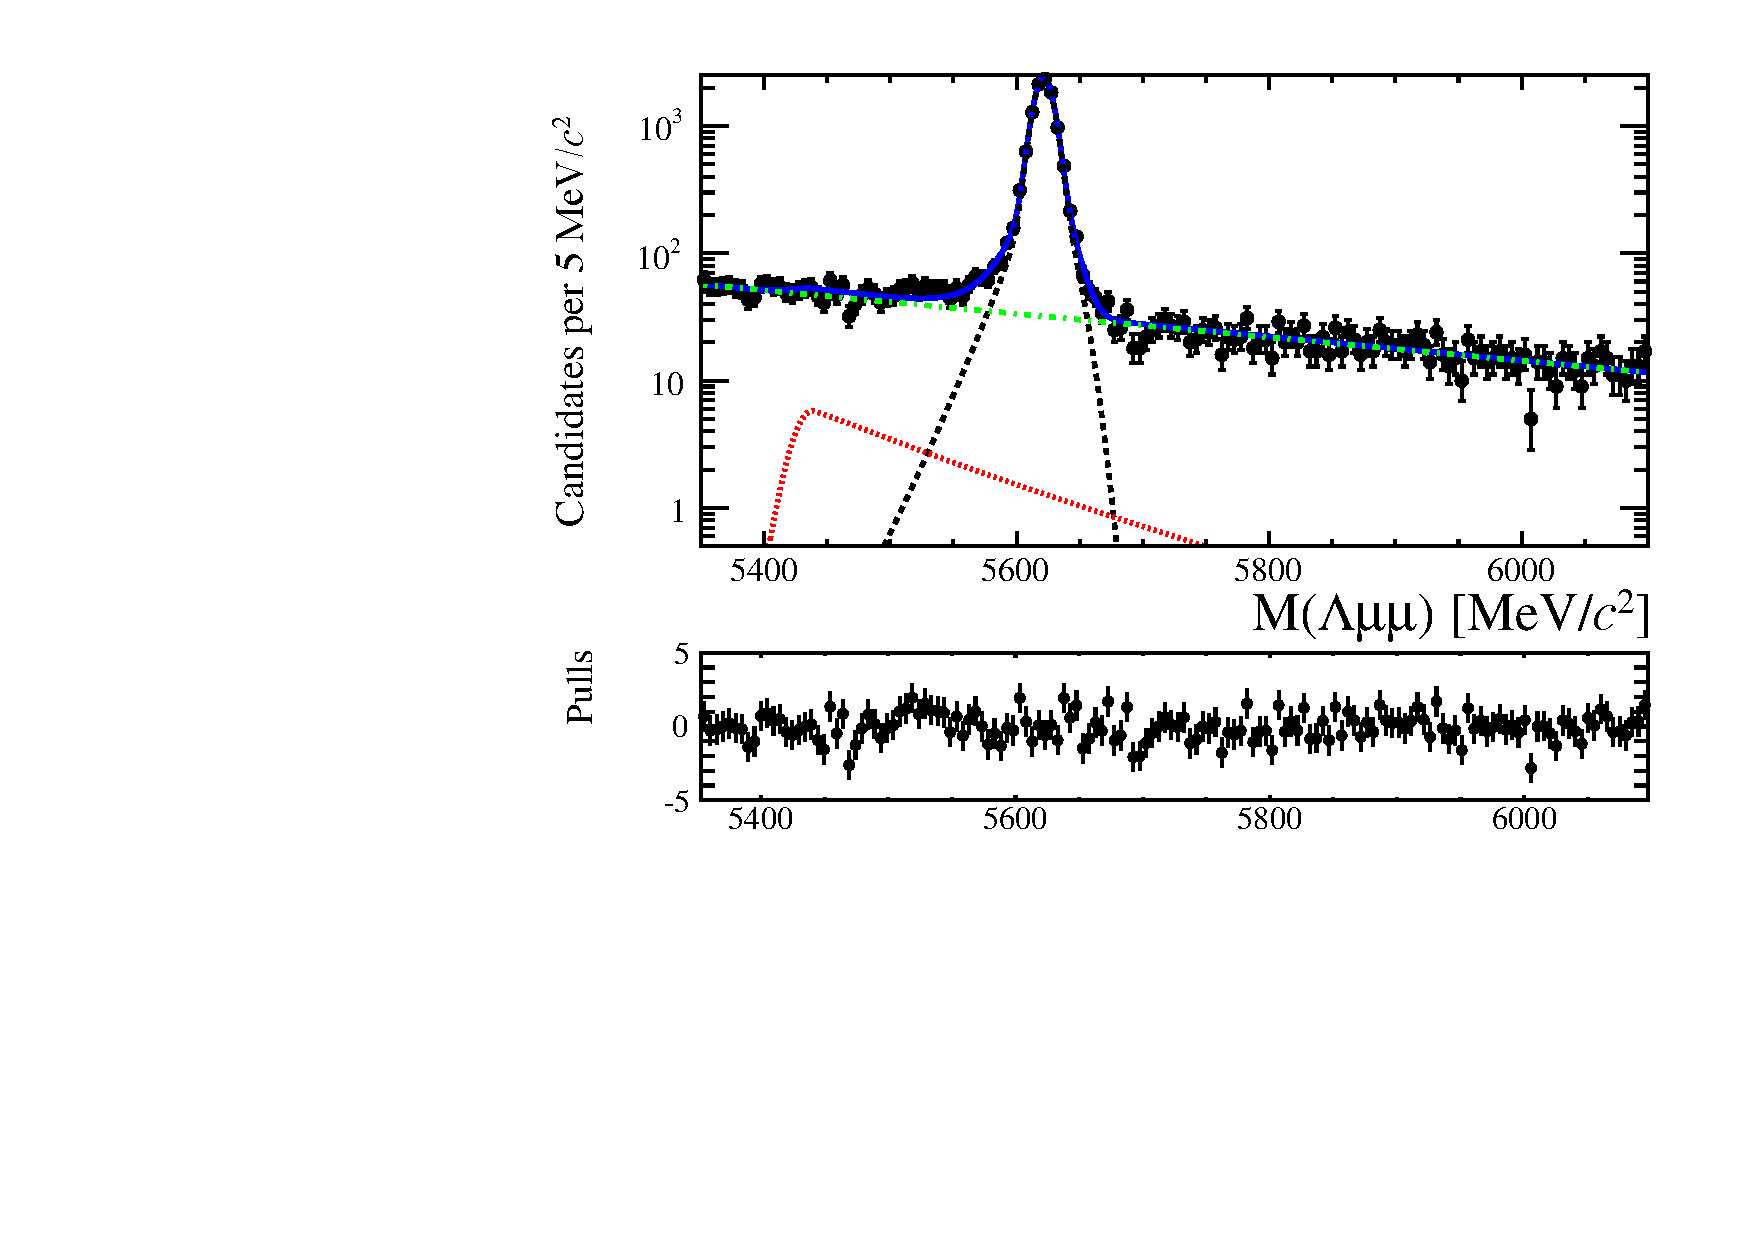
\includegraphics[width=0.48\textwidth]{Lmumu/figs/Jpsi_default_DD_log_fitAndRes.pdf}
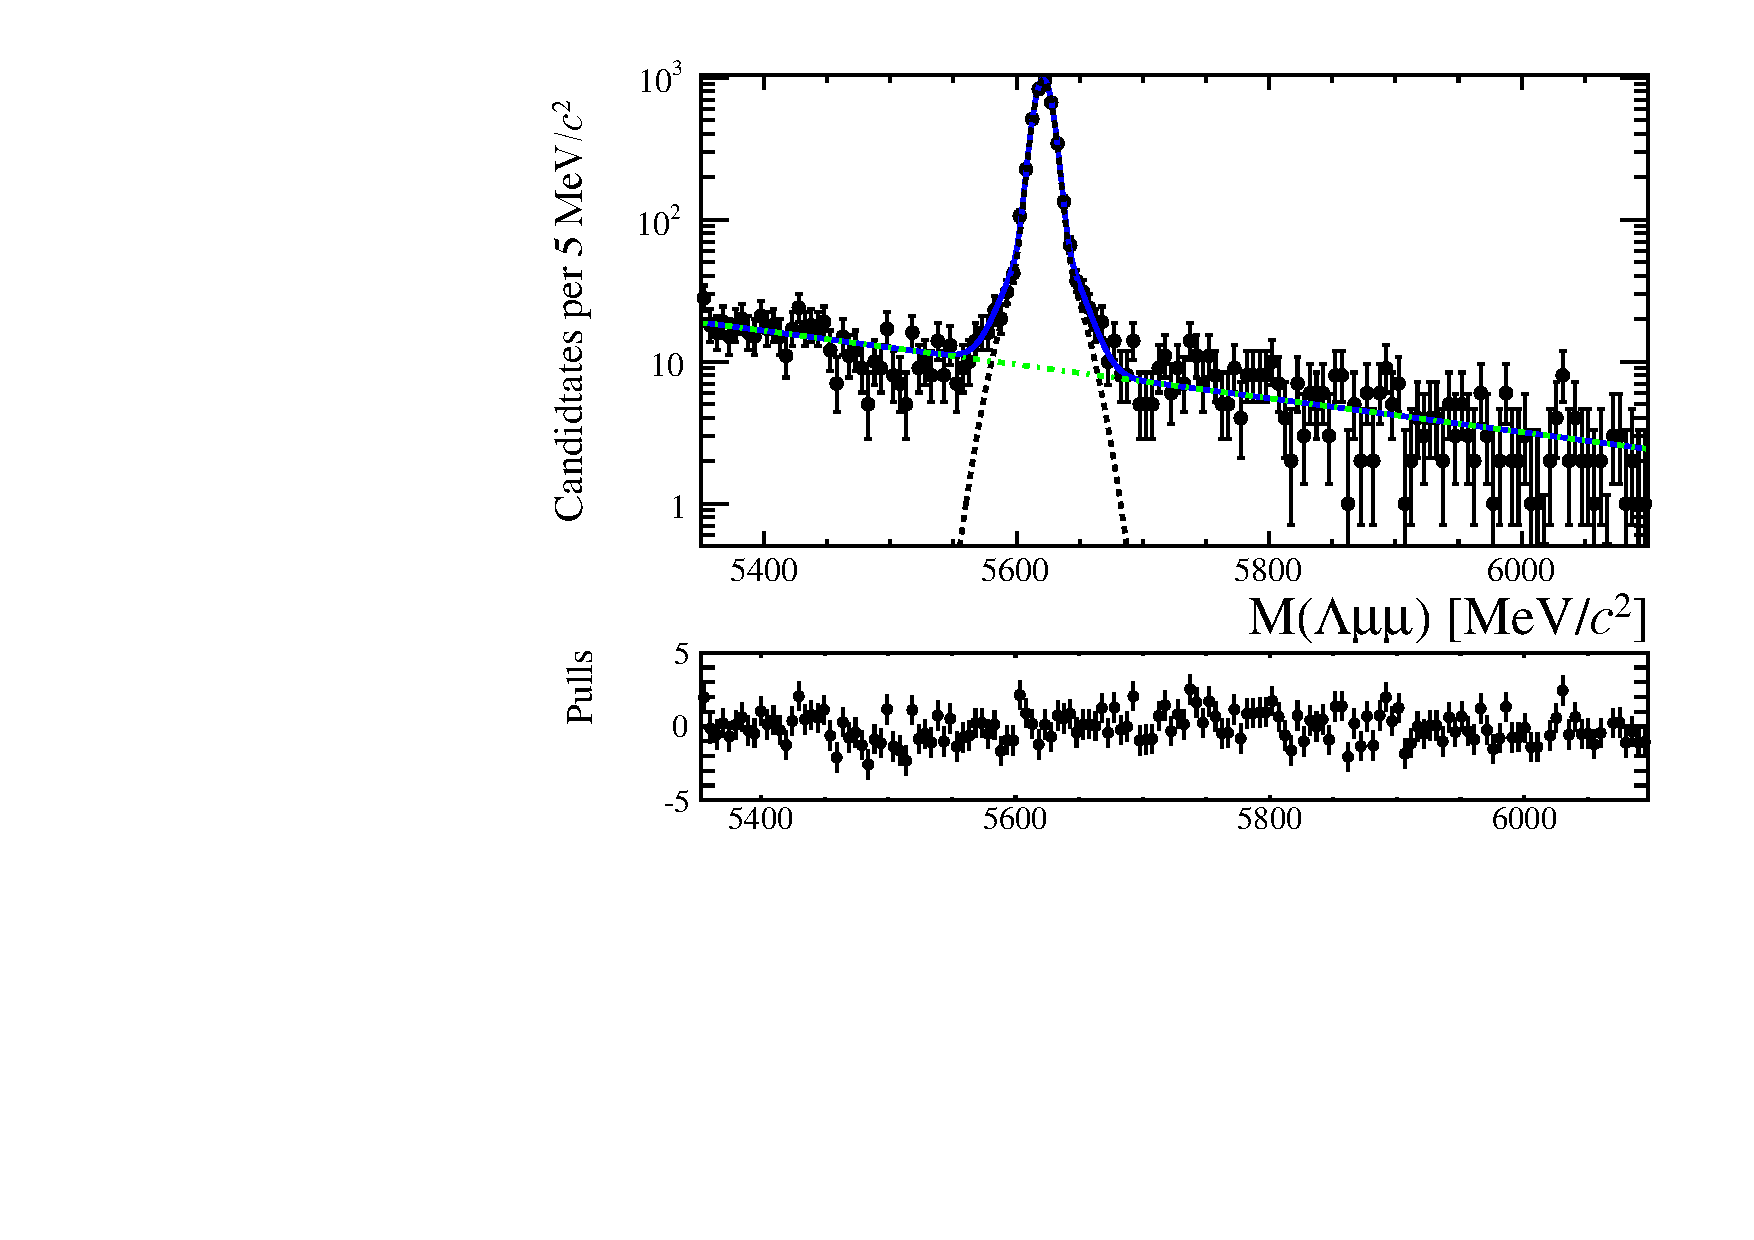
\includegraphics[width=0.48\textwidth]{Lmumu/figs/Jpsi_default_LL_log_fitAndRes.pdf}
\caption{Invariant mass distribution of \Lb\ra\jpsi\Lz downstream (left) and long (right)
candidates with an extra proton PID cut to remove \KS background. }
\label{fig:Jpsimass_angular}
\end{figure}
%
\begin{figure}[h]
\centering
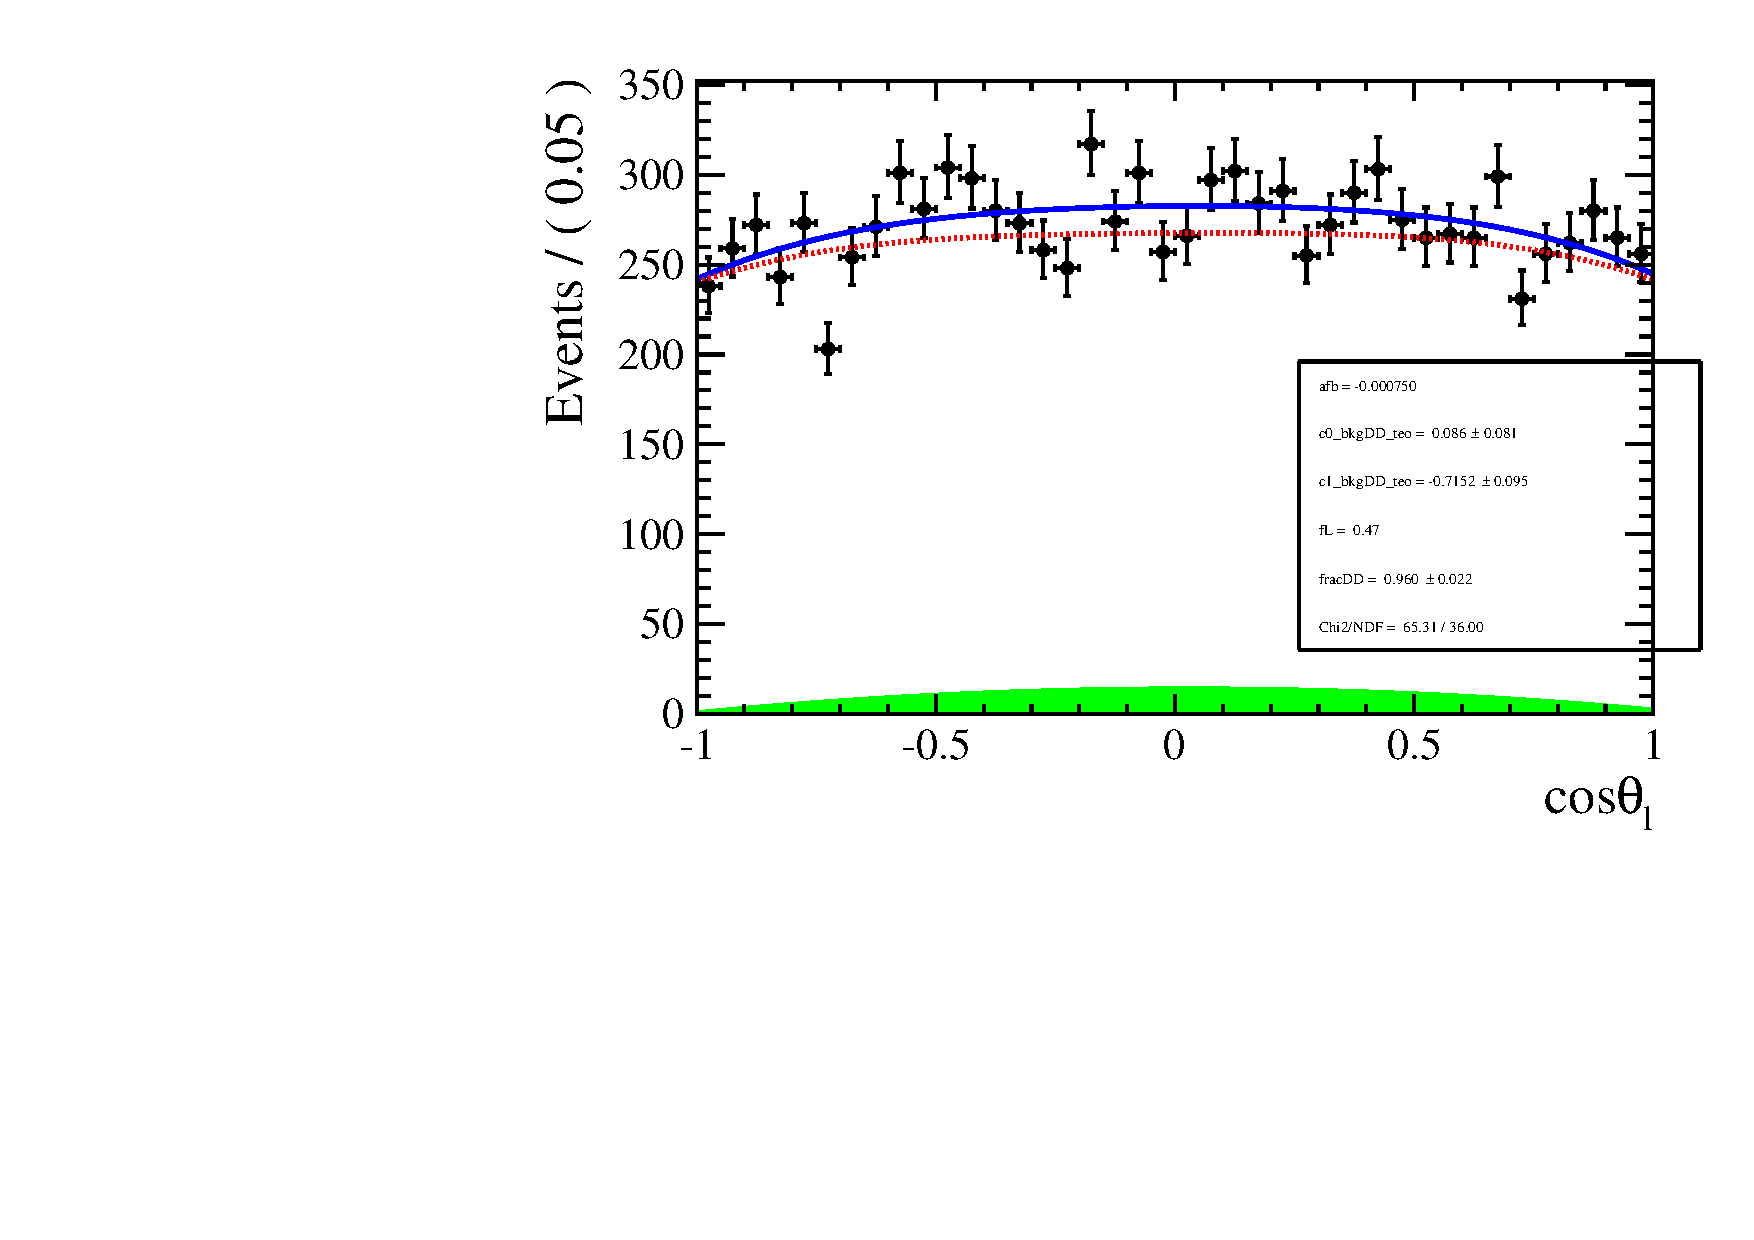
\includegraphics[width=0.48\textwidth]{Lmumu/figs/AngularDistribs/Fitted/Afb_DD_jpsi.pdf}
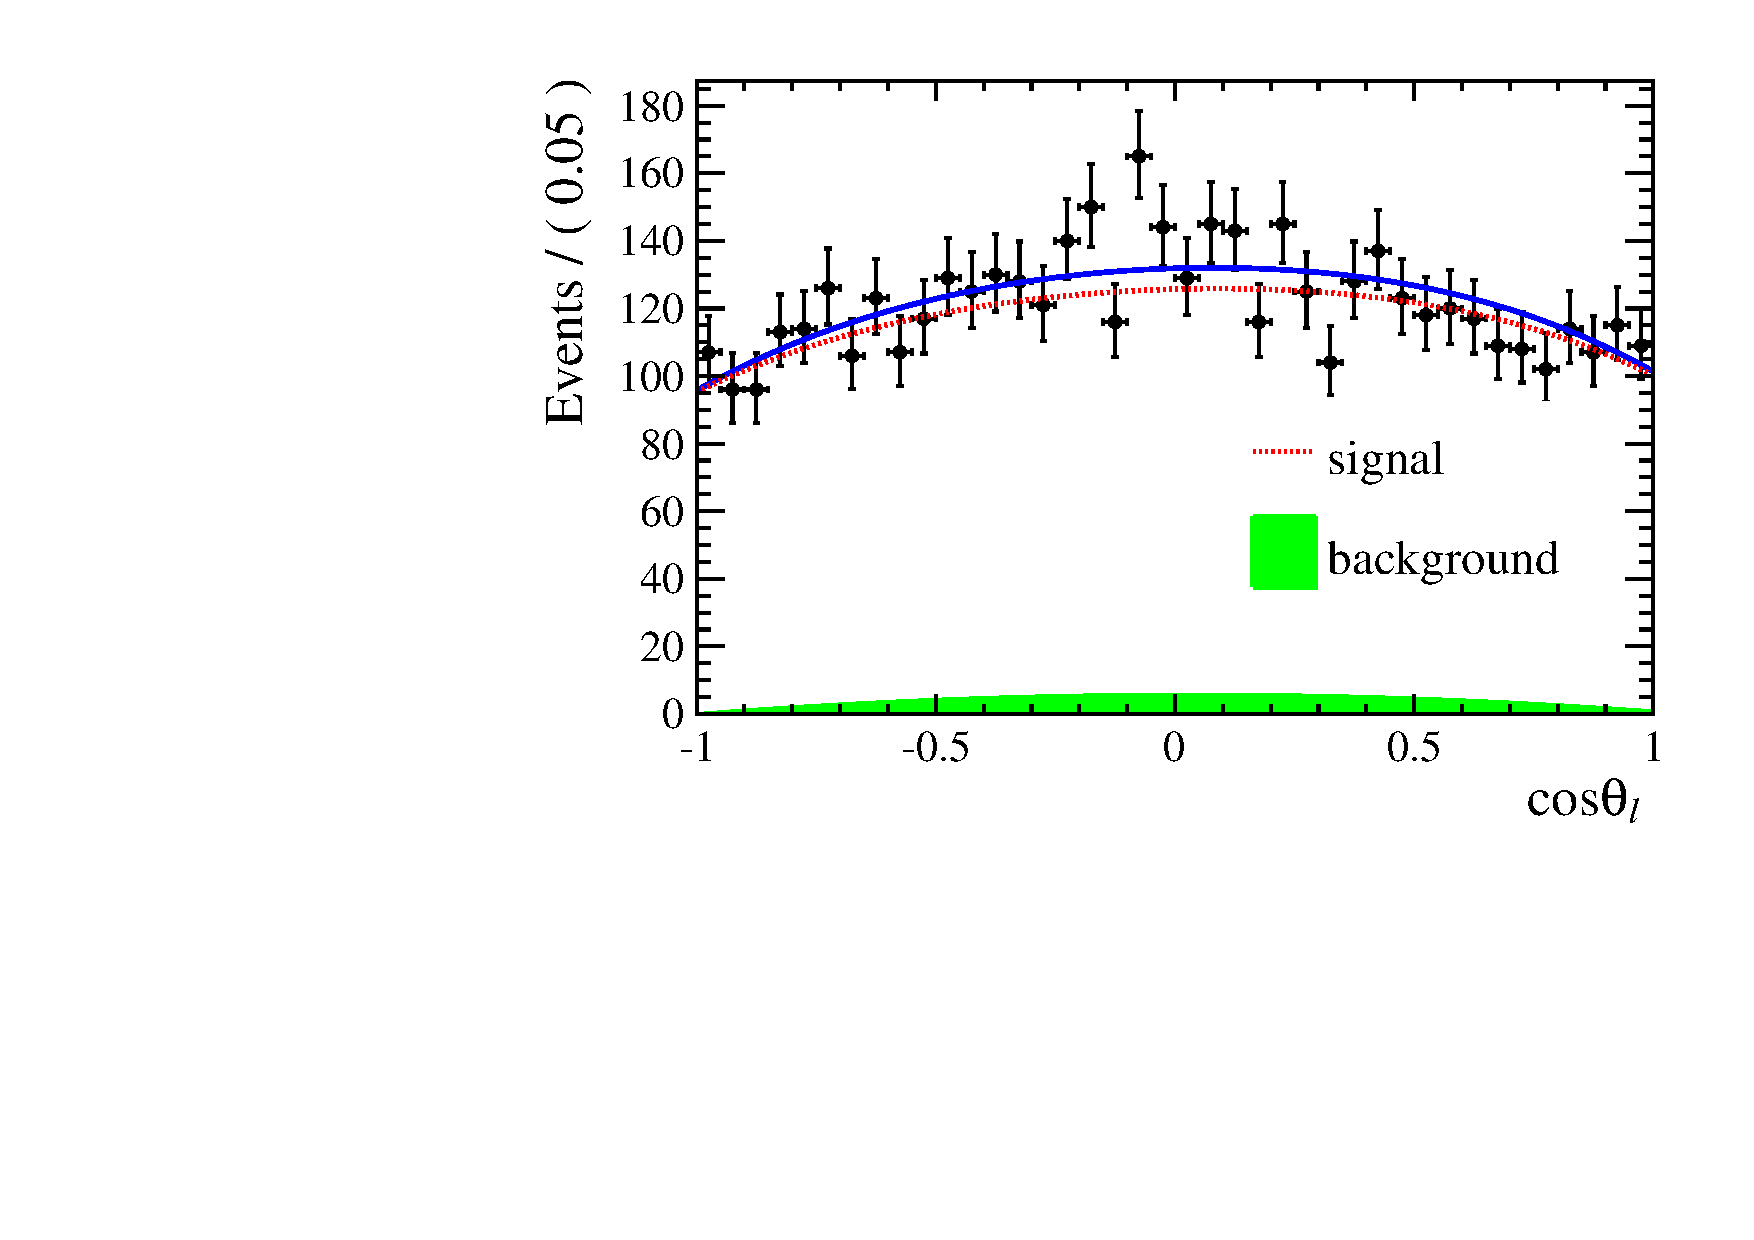
\includegraphics[width=0.48\textwidth]{Lmumu/figs/AngularDistribs/Fitted/Afb_LL_jpsi.pdf}
\caption{Fitted $\cos\theta_\ell$ angular distribution for $\Lb\to\jpsi\Lz$ candidates
reconstructed using downstream (left) and long (right) tracks. }
\label{fig:AngFitJpsi}
\end{figure}
%
\begin{figure}[h]
\centering
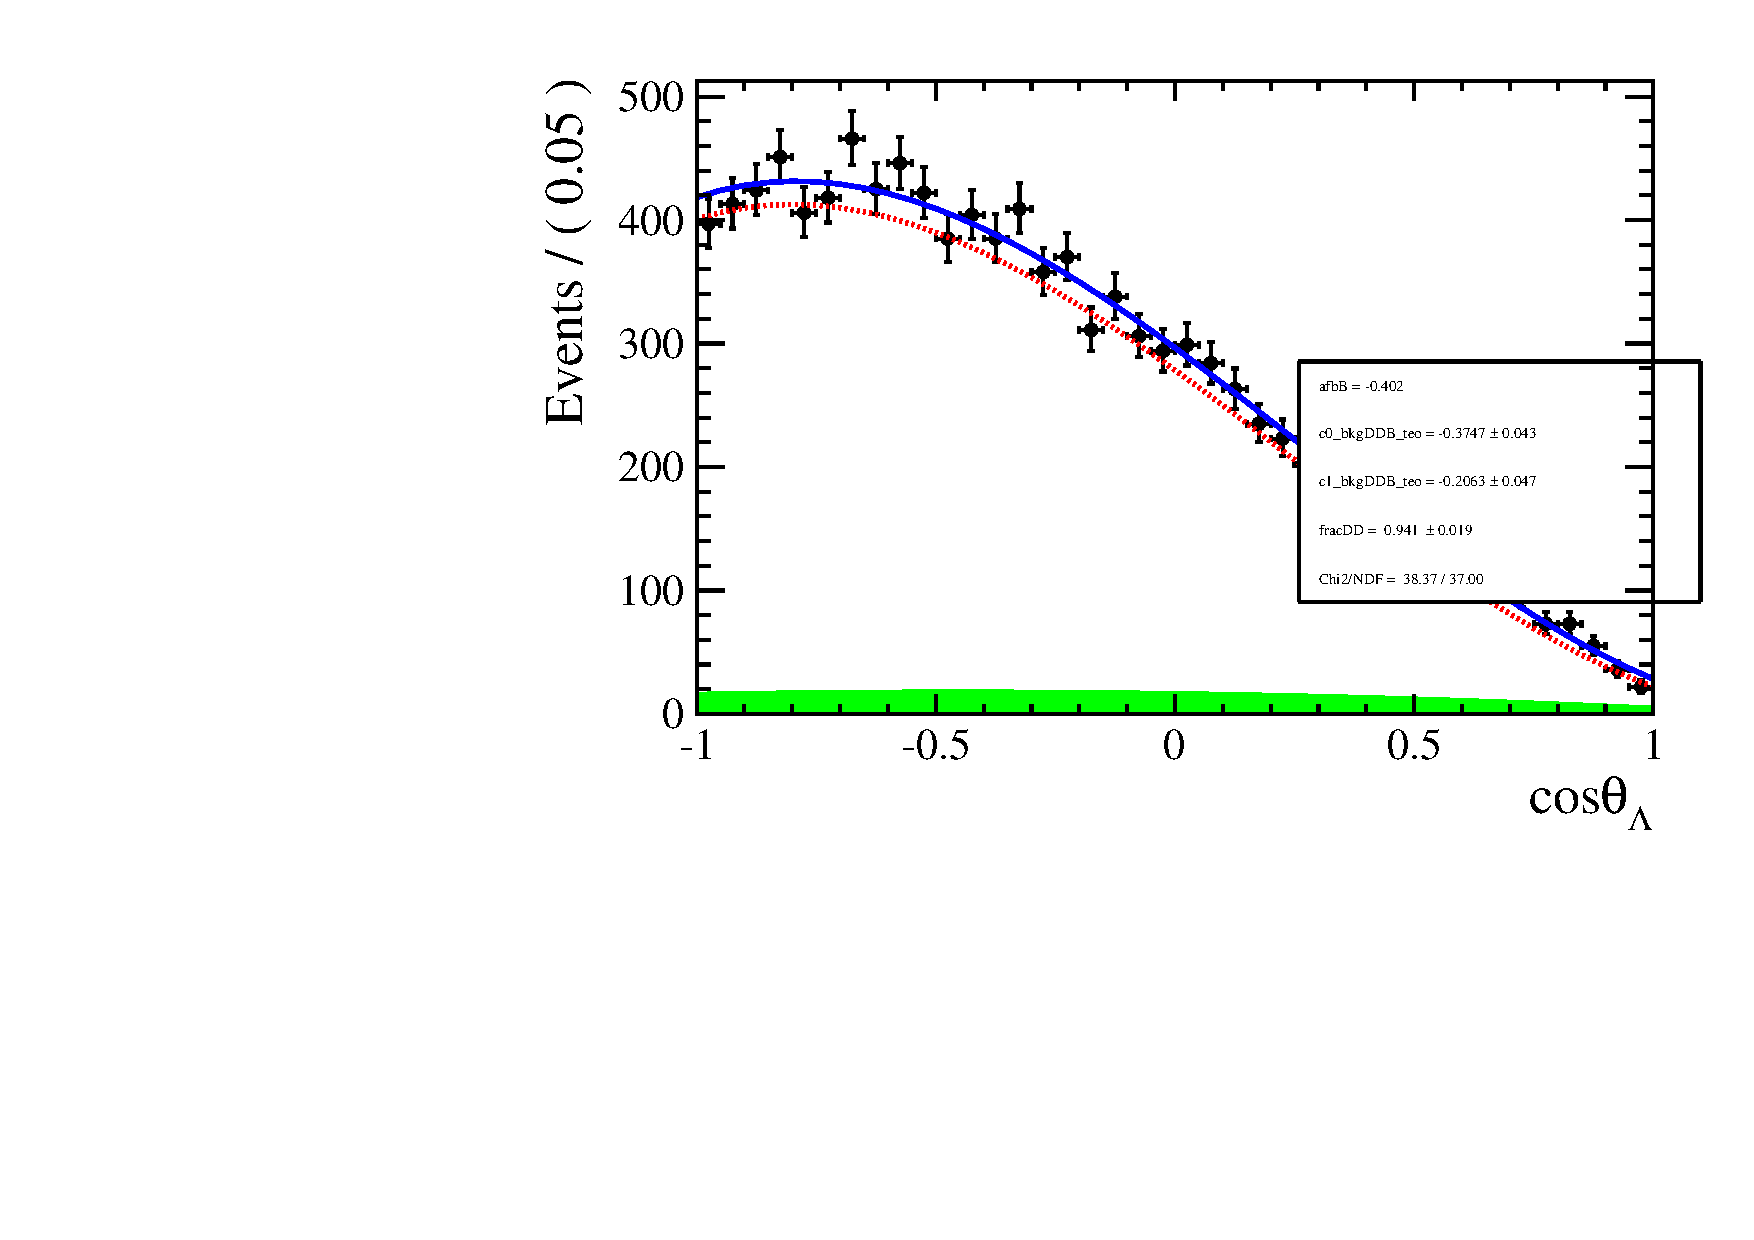
\includegraphics[width=0.48\textwidth]{Lmumu/figs/AngularDistribs/Fitted/AfbB_DD_jpsi.pdf}
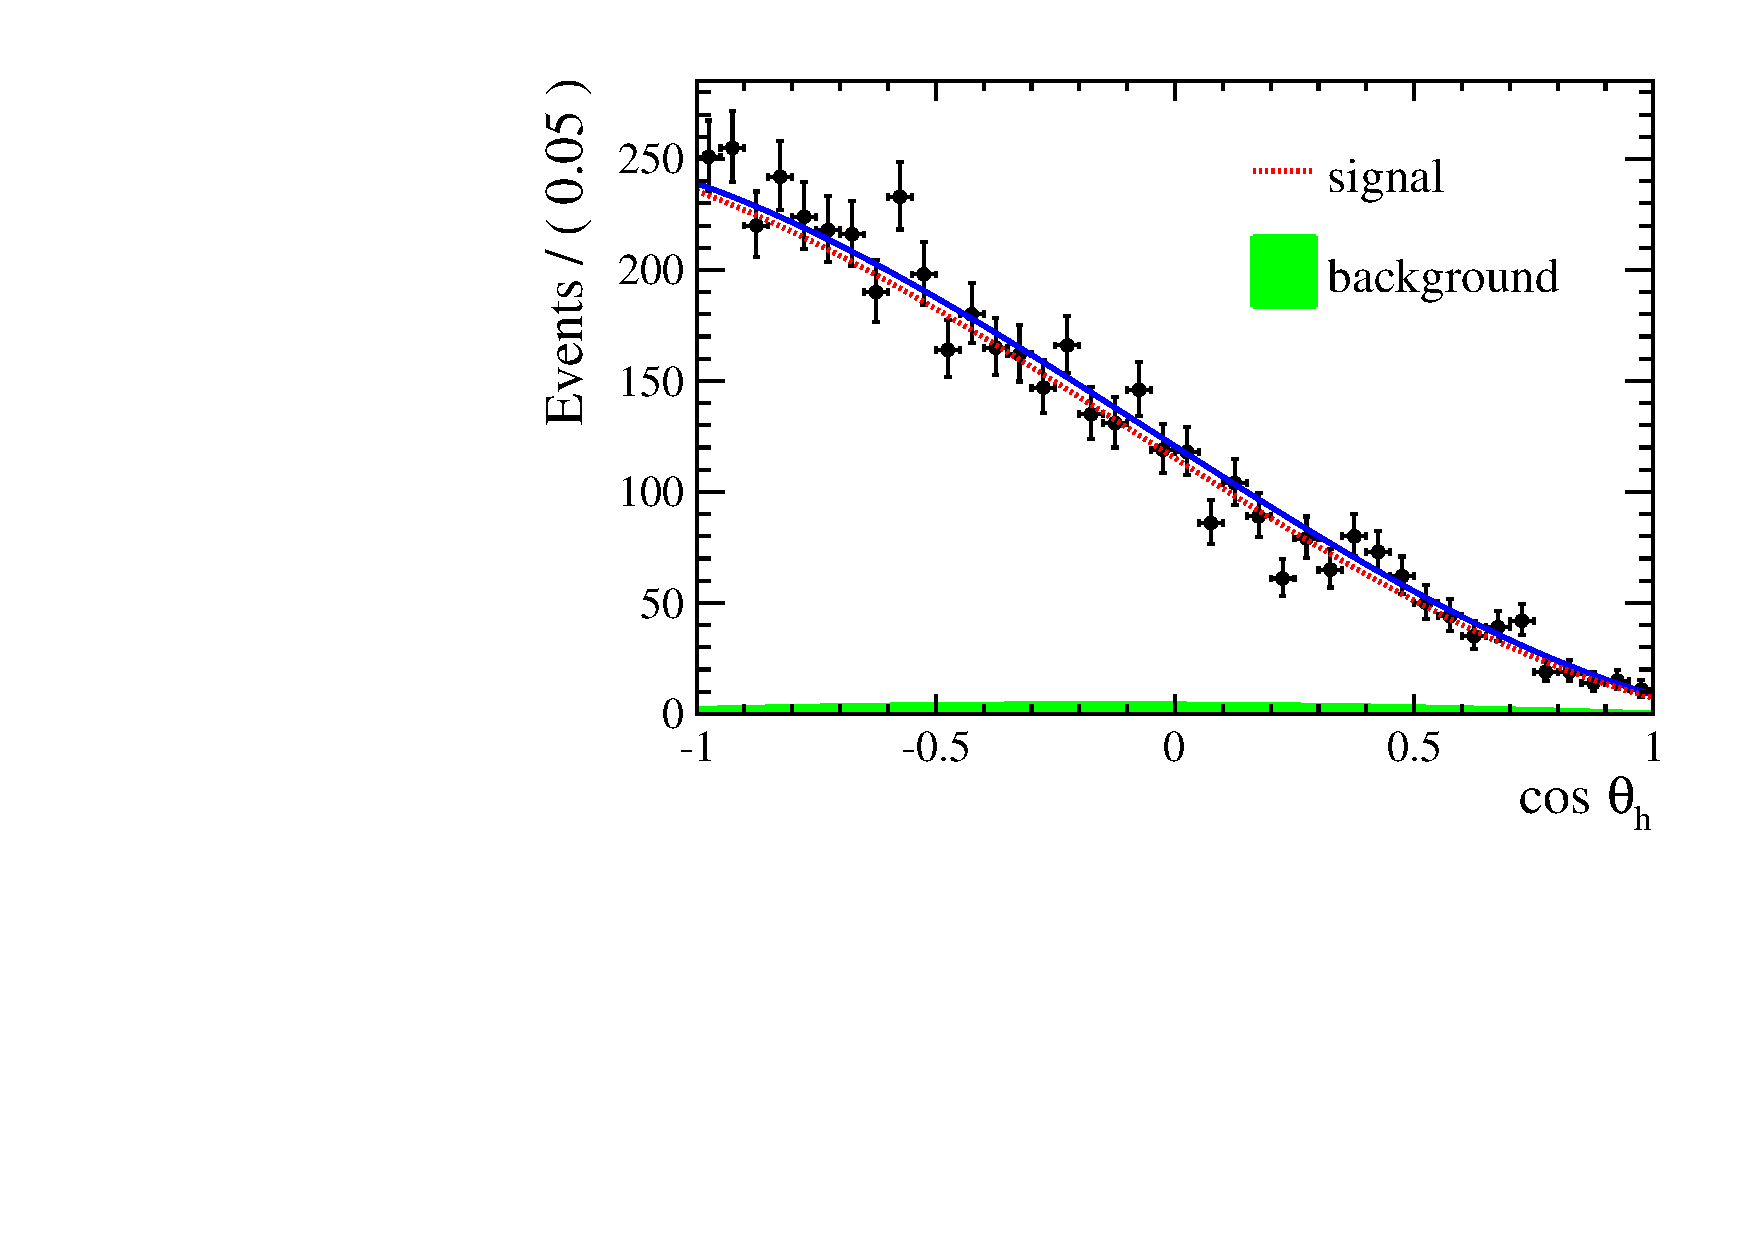
\includegraphics[width=0.48\textwidth]{Lmumu/figs/AngularDistribs/Fitted/AfbB_LL_jpsi.pdf}
\caption{Fitted $\cos\theta_h$ angular distribution for $\Lb\to\jpsi\Lz$ candidates
reconstructed using downstream (left) and long (right) tracks.  }
\label{fig:AngFitBJpsi}
\end{figure}
%
The signal model used for the angular fit to $\Lb\to\jpsi\Lz$ candidates is the same defined
 for the rare case and described in Sec.~\ref{sec:angfit}.
For the background instead the higher statistics allows to leave more freedom to the fit.
Therefore a second-order Chebyschev polynomial is used, where the two parameters are
free to vary. As for the rare case the background fractions are gaussian-constrained
to what found from the invariant mass fit. Figures~\ref{fig:AngFitJpsi} and~\ref{fig:AngFitBJpsi} show
fitted angular distributions for the \jpsi channel. The measured values of the observables
are \mbox{$\afbl = -0.002^{+0.011}_{-0.011}$}, $\afbh = -0.402^{+0.010}_{-0.009}$
and $\fl = 0.485^{+0.019}_{-0.020}$, where the uncertainties are 68\% Feldman-Cousins 
confidence intervals. The lepton side asymmetry is measured to be zero 
as expected for a tree level $\bquark\to\cquark\cquarkbar\squark$ process.






\section{Results}
\label{sec:afb_results}

Figures~\ref{fig:AngFit} and~\ref{fig:AngFitB} show fits to the angular distributions
for the 15 -- 20~\gevgevcccc ~\qsq interval and 
%The LL and DD distributions are fitted simultaneously and therefore we only have two free parameters
%in the fit, $\fl$ and $\afbl$, for the lepton side and one, $\afbh$, for the hadron one.
%
Tab.~\ref{tab:angresults} reports measured values of $\afbl$, $\afbh$ and $\fl$ in all intervals.
The asymmetries are also shown in Fig.~\ref{fig:Afb_results} together with SM predictions obtained from 
Ref.~\cite{Detmold:2012vy}. The statistical uncertainties on these tables 
are obtained using the likelihood-ratio ordering method described in Sec.~\ref{sec:FeldmanCousins}, where only
one of the two observables is treated as the PoI at a time. The statistical uncertainties
on $\afbl$ and $\fl$ are also reported in Fig.~\ref{fig:contours} as two-dimensional 68\;\% confidence level regions,
where the likelihood-ratio ordering method is applied by varying both observables at the same time and therefore taking
correlations into account. Total systematic uncertainties correspond to the square root sum of the
single considered sources.

\begin{figure}[t]
\centering
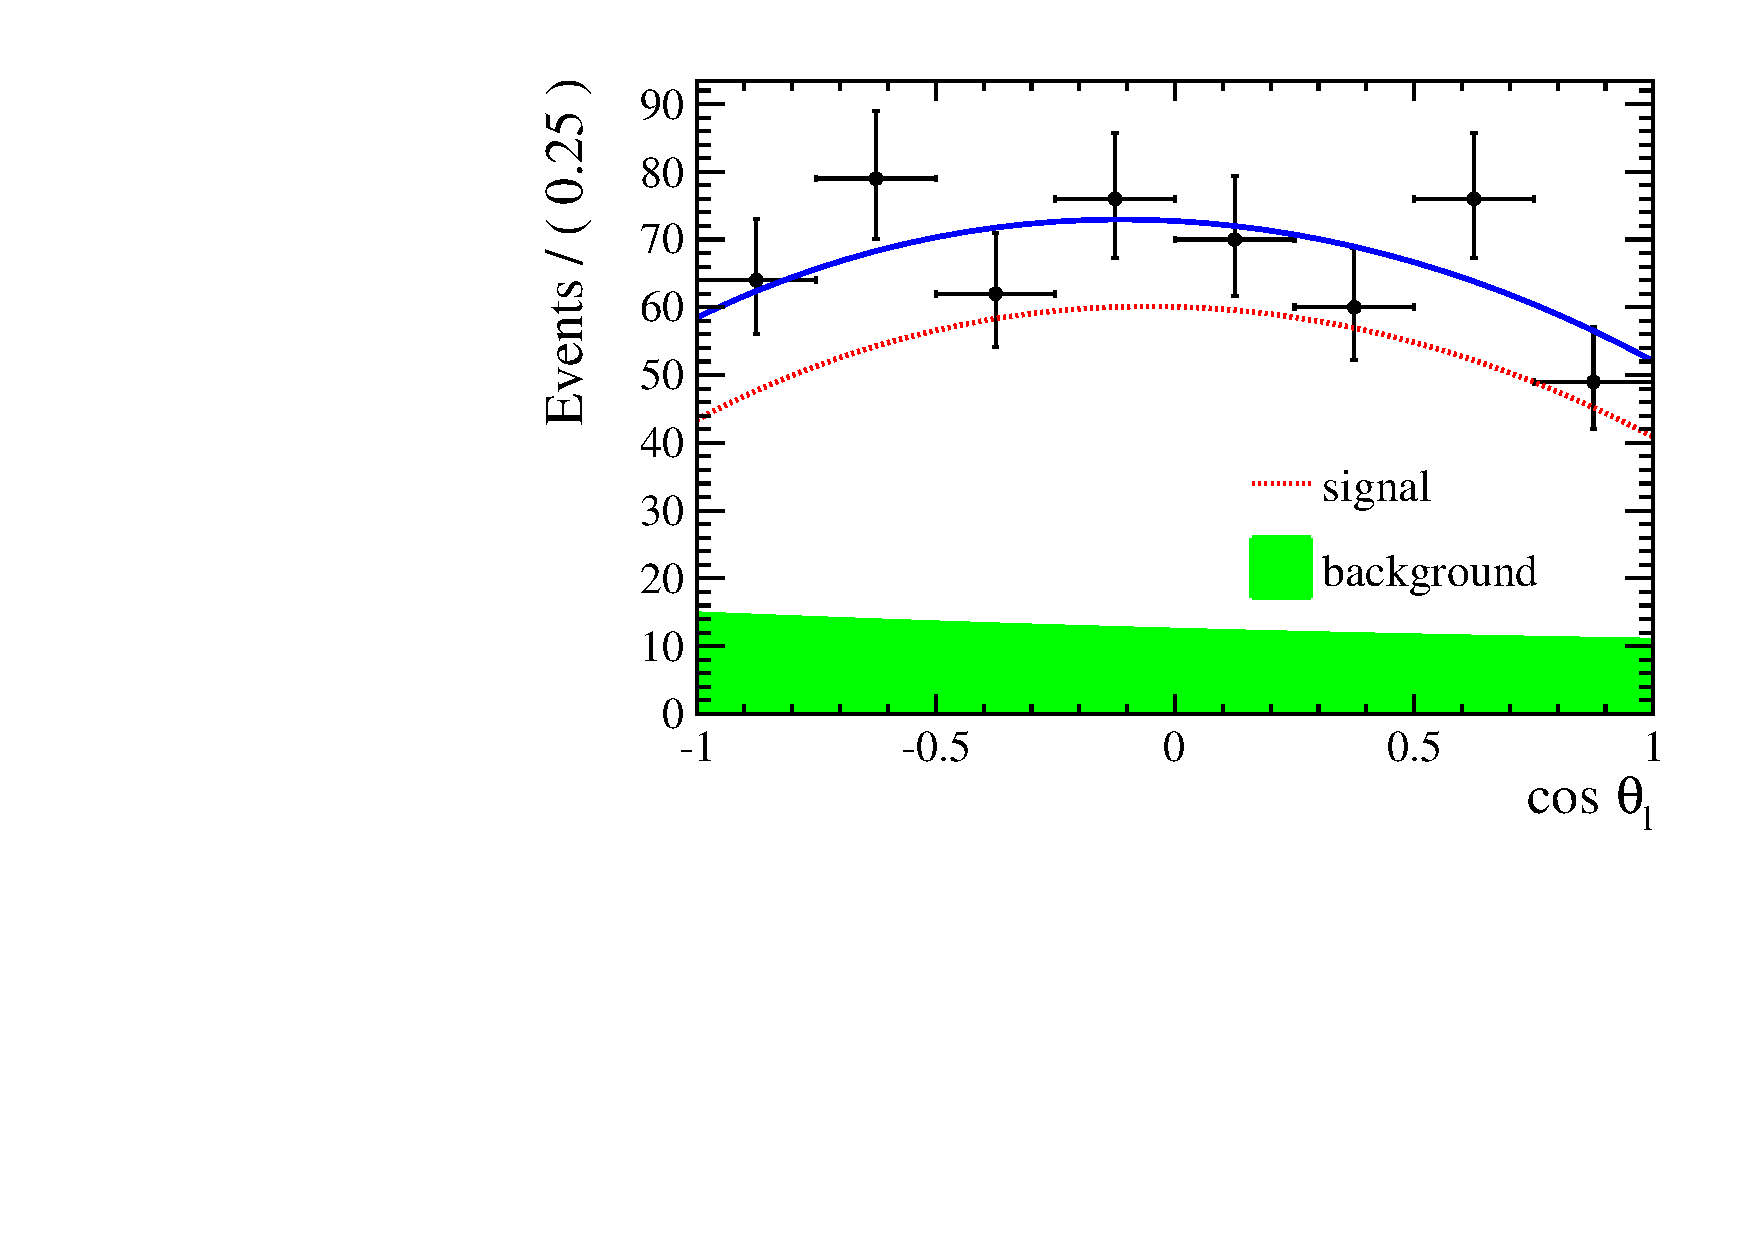
\includegraphics[width=0.48\textwidth]{Lmumu/figs/AngularDistribs/Fitted/Afb_DD_q2_1500_2000.pdf}
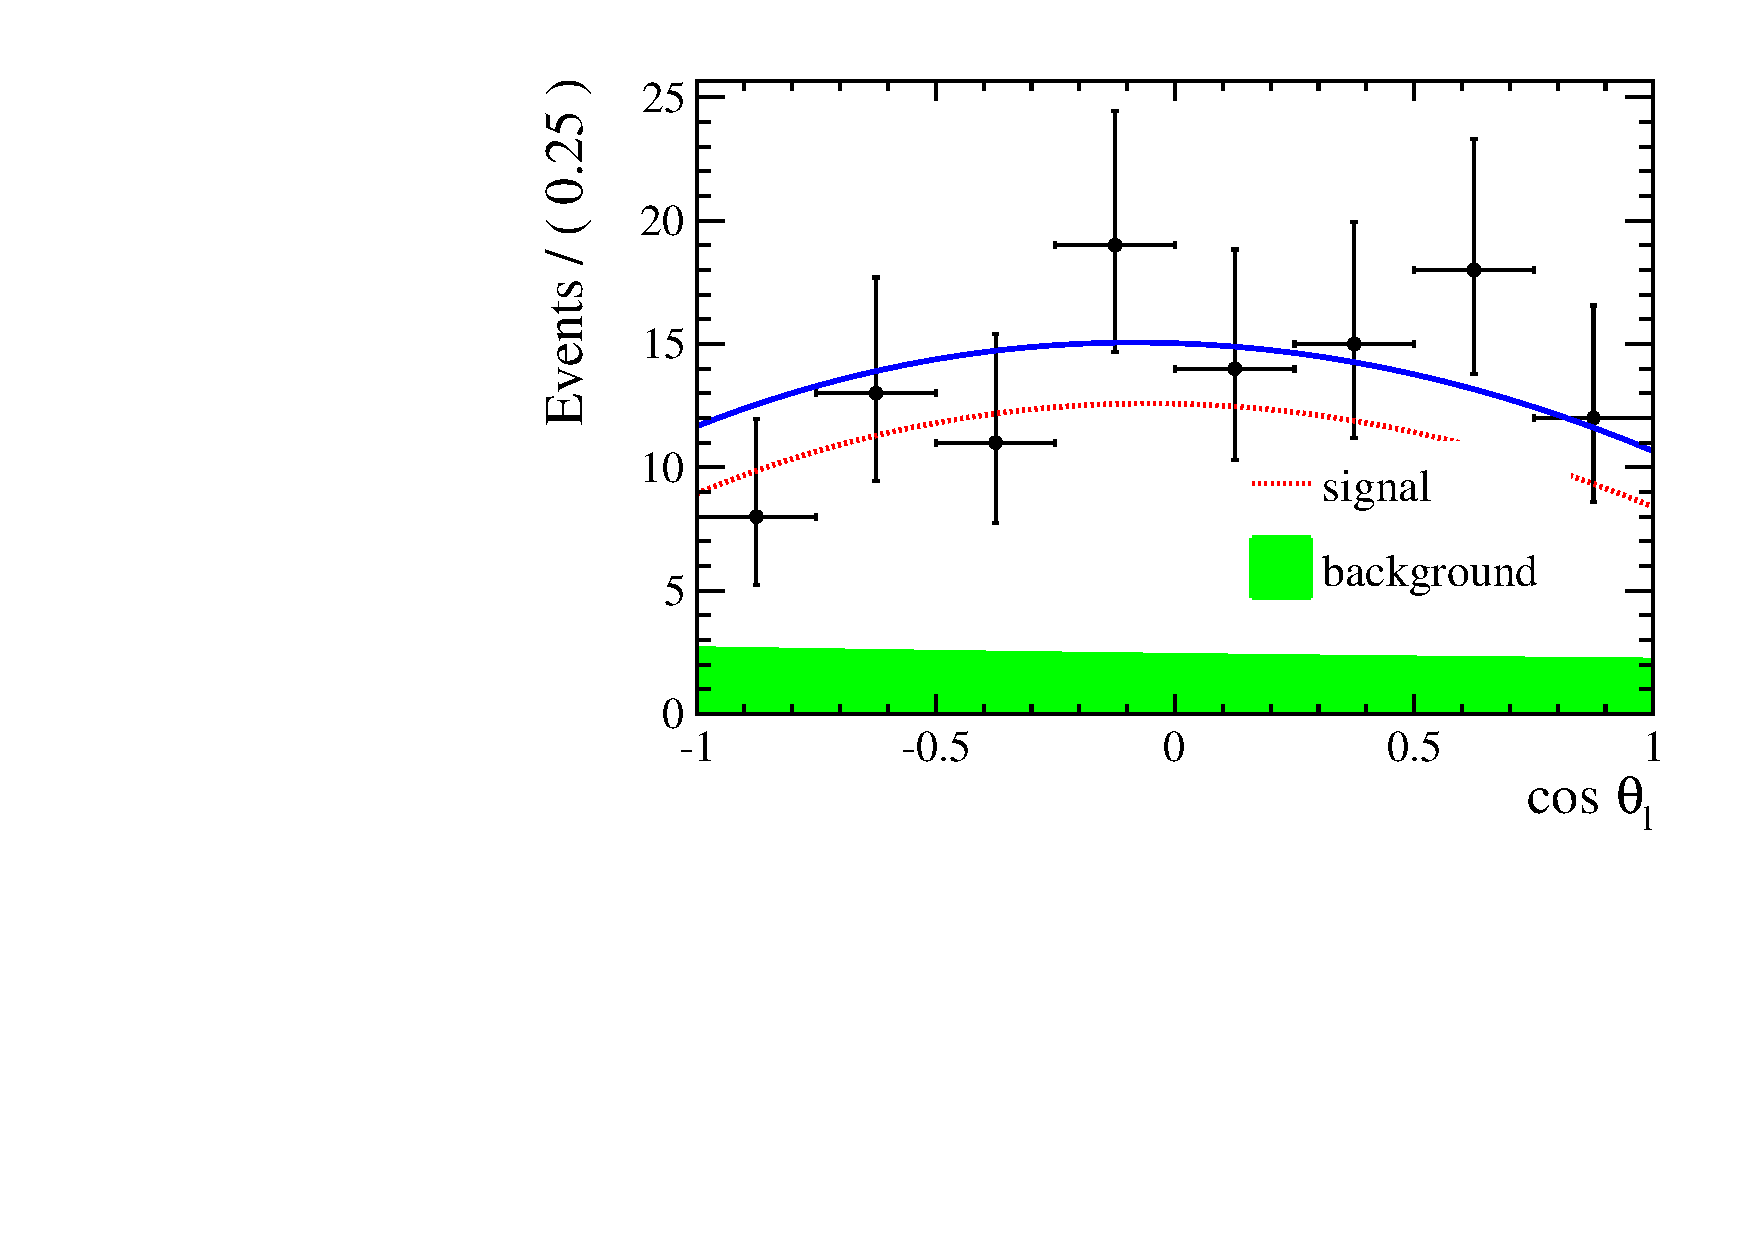
\includegraphics[width=0.48\textwidth]{Lmumu/figs/AngularDistribs/Fitted/Afb_LL_q2_1500_2000.pdf}
\caption{Fitted $\cos\theta_\ell$ angular distributions for downstream
 (left) and long (right) candidates in the 15 -- 20~\gevgevcccc ~\qsq interval.  }
\label{fig:AngFit}
\end{figure}
%
\begin{figure}[h]
\centering
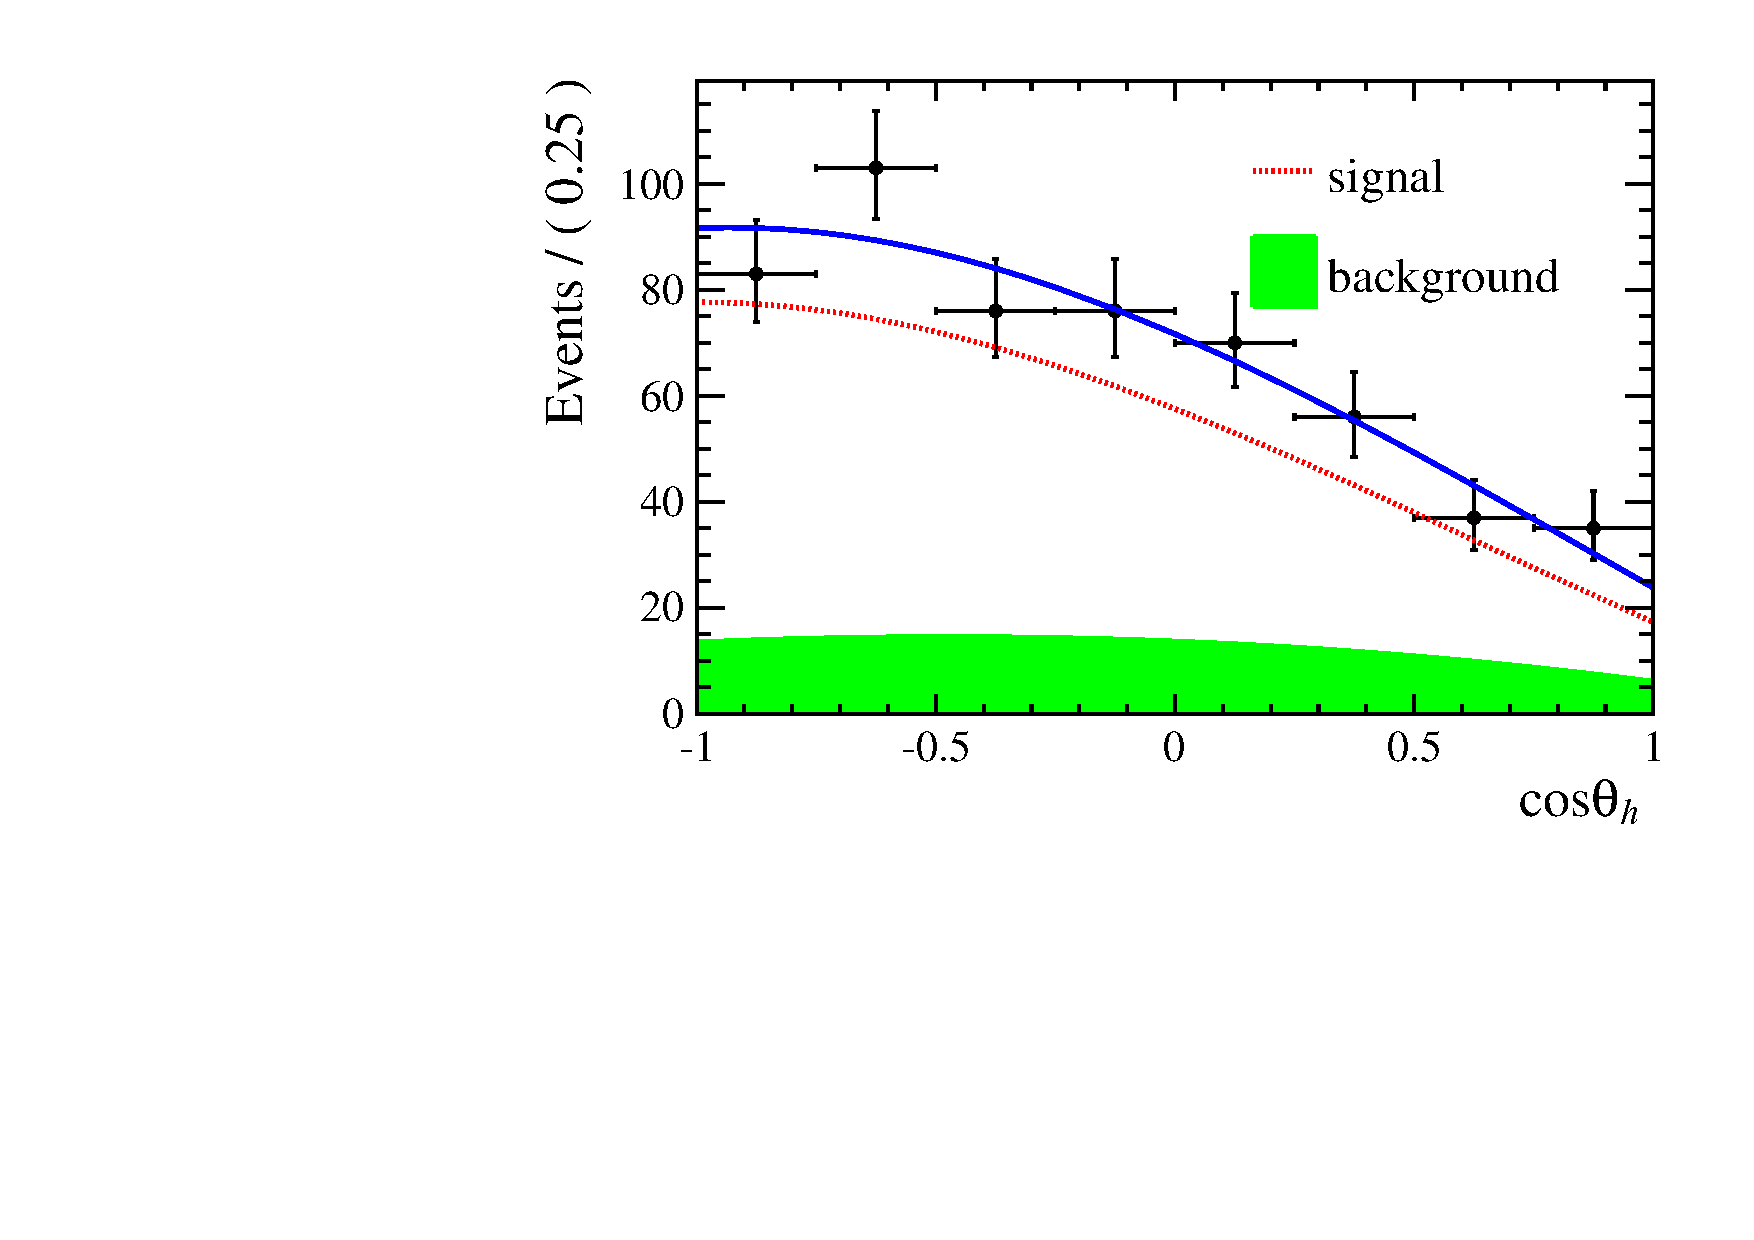
\includegraphics[width=0.48\textwidth]{Lmumu/figs/AngularDistribs/Fitted/AfbB_DD_q2_1500_2000.pdf}
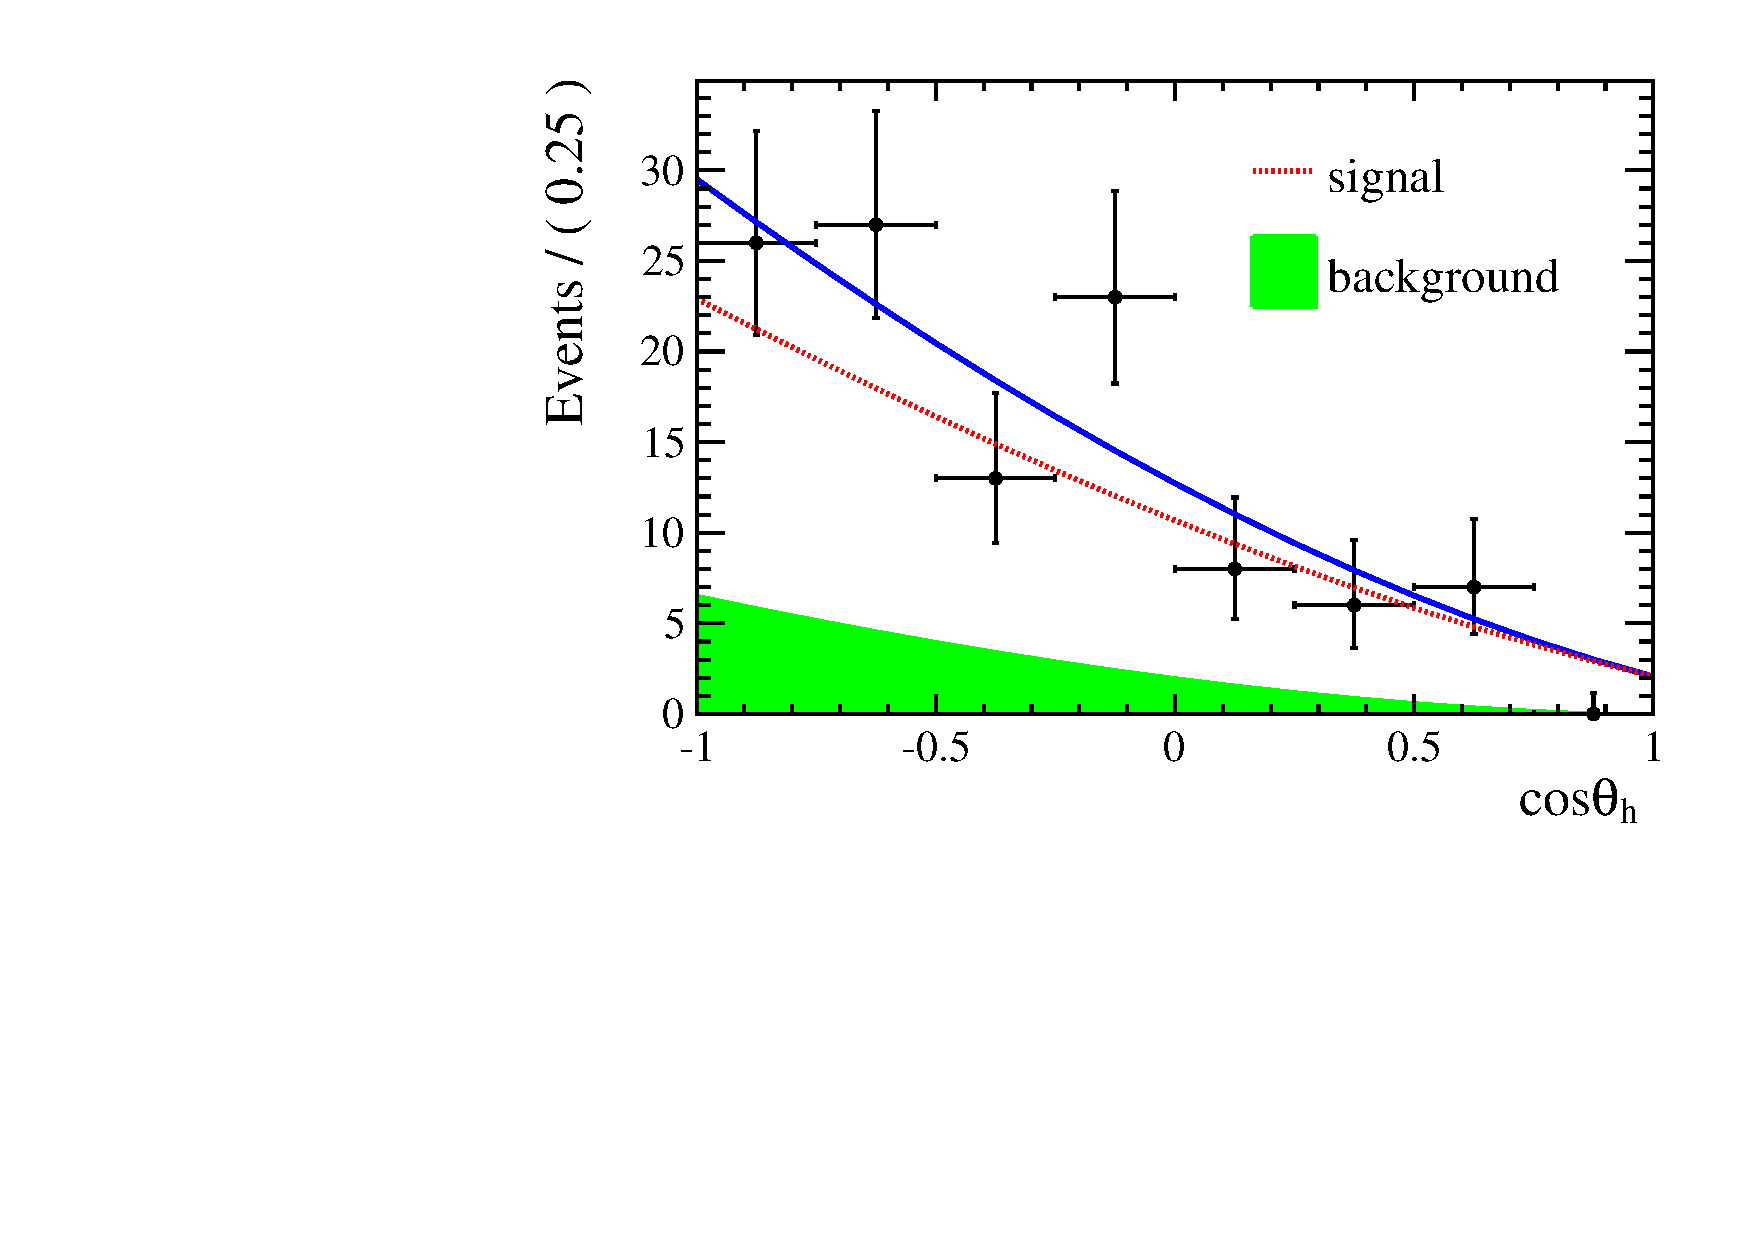
\includegraphics[width=0.48\textwidth]{Lmumu/figs/AngularDistribs/Fitted/AfbB_LL_q2_1500_2000.pdf}
\caption{Fitted $\cos\theta_h$ angular distributions for downstream
 (left) and long (right) candidates in the 15 -- 20~\gevgevcccc ~\qsq interval.  }
 \label{fig:AngFitB}
\end{figure}
%
\begin{table}[h!]
\centering
\caption{Measured values of leptonic and hadronic angular observables;
uncertainties are statistical and systematic.}
\label{tab:angresults}
\renewcommand{\arraystretch}{1.2}
\begin{tabular}{$c|^c^c^c}
\rowstyle{\bfseries}
\boldmath{ \qsq  [\gevgevcccc]}   &            \boldmath{\afbl}      &   \boldmath{    \fl 	}			& \boldmath{ \afbh     }           \\ \hline

0.1 -- 2.0   & $\phantom{-\,}0.37 \; ^{+\;0.37}_{-\;0.48} \,\pm\, 0.03$  	&   $0.56 \; ^{+\;0.23}_{-\;0.56}\,\pm\, 0.08$ 		& $-\;0.12 \; ^{+\;0.31}_{-\;0.28}\,\pm\, 0.15$	\\
11.0 -- 12.5 & $\phantom{-\,}0.01 \; ^{+\;0.19}_{-\;0.18} \,\pm\, 0.06$  	&   $0.40 \; ^{+\;0.37}_{-\;0.36}\,\pm\, 0.06$		& $-\;0.50 \; ^{+\;0.10}_{-\;0.00}\,\pm\, 0.04$	 \\
15.0 -- 16.0 & $-\,0.10 \; ^{+\;0.18}_{-\;0.16} \,\pm\, 0.03$  			&   $0.49 \; ^{+\;0.30}_{-\;0.30} \,\pm\, 0.05$ 	& $-\;0.19 \; ^{+\;0.14}_{-\;0.16}\,\pm\, 0.03$	\\	
16.0 -- 18.0 & $-\,0.07 \; ^{+\;0.13}_{-\;0.12} \,\pm\, 0.04$  			&   $0.68 \; ^{+\;0.15}_{-\;0.21} \,\pm\, 0.05$ 	& $-\;0.44 \; ^{+\;0.10}_{-\;0.05}\,\pm\, 0.03$	\\
18.0 -- 20.0 & $\phantom{-\,}0.01 \; ^{+\;0.15}_{-\;0.14} \,\pm\; 0.04$  	&   $0.62 \; ^{+\;0.24}_{-\;0.27}\,\pm\, 0.04$ 		& $-\;0.13 \; ^{+\;0.09}_{-\;0.12}\,\pm\, 0.03$	\\ \hline
15.0 -- 20.0 & $-\,0.05 \; ^{+\;0.09}_{-\;0.09} \,\pm\, 0.03$  			&   $0.61 \; ^{+\;0.11}_{-\;0.14} \,\pm\, 0.03$ 	& $-\;0.29 \; ^{+\;0.07}_{-\;0.07}\,\pm\, 0.03$	\\
\end{tabular}
\end{table}

\begin{figure}[ptb]
\centering
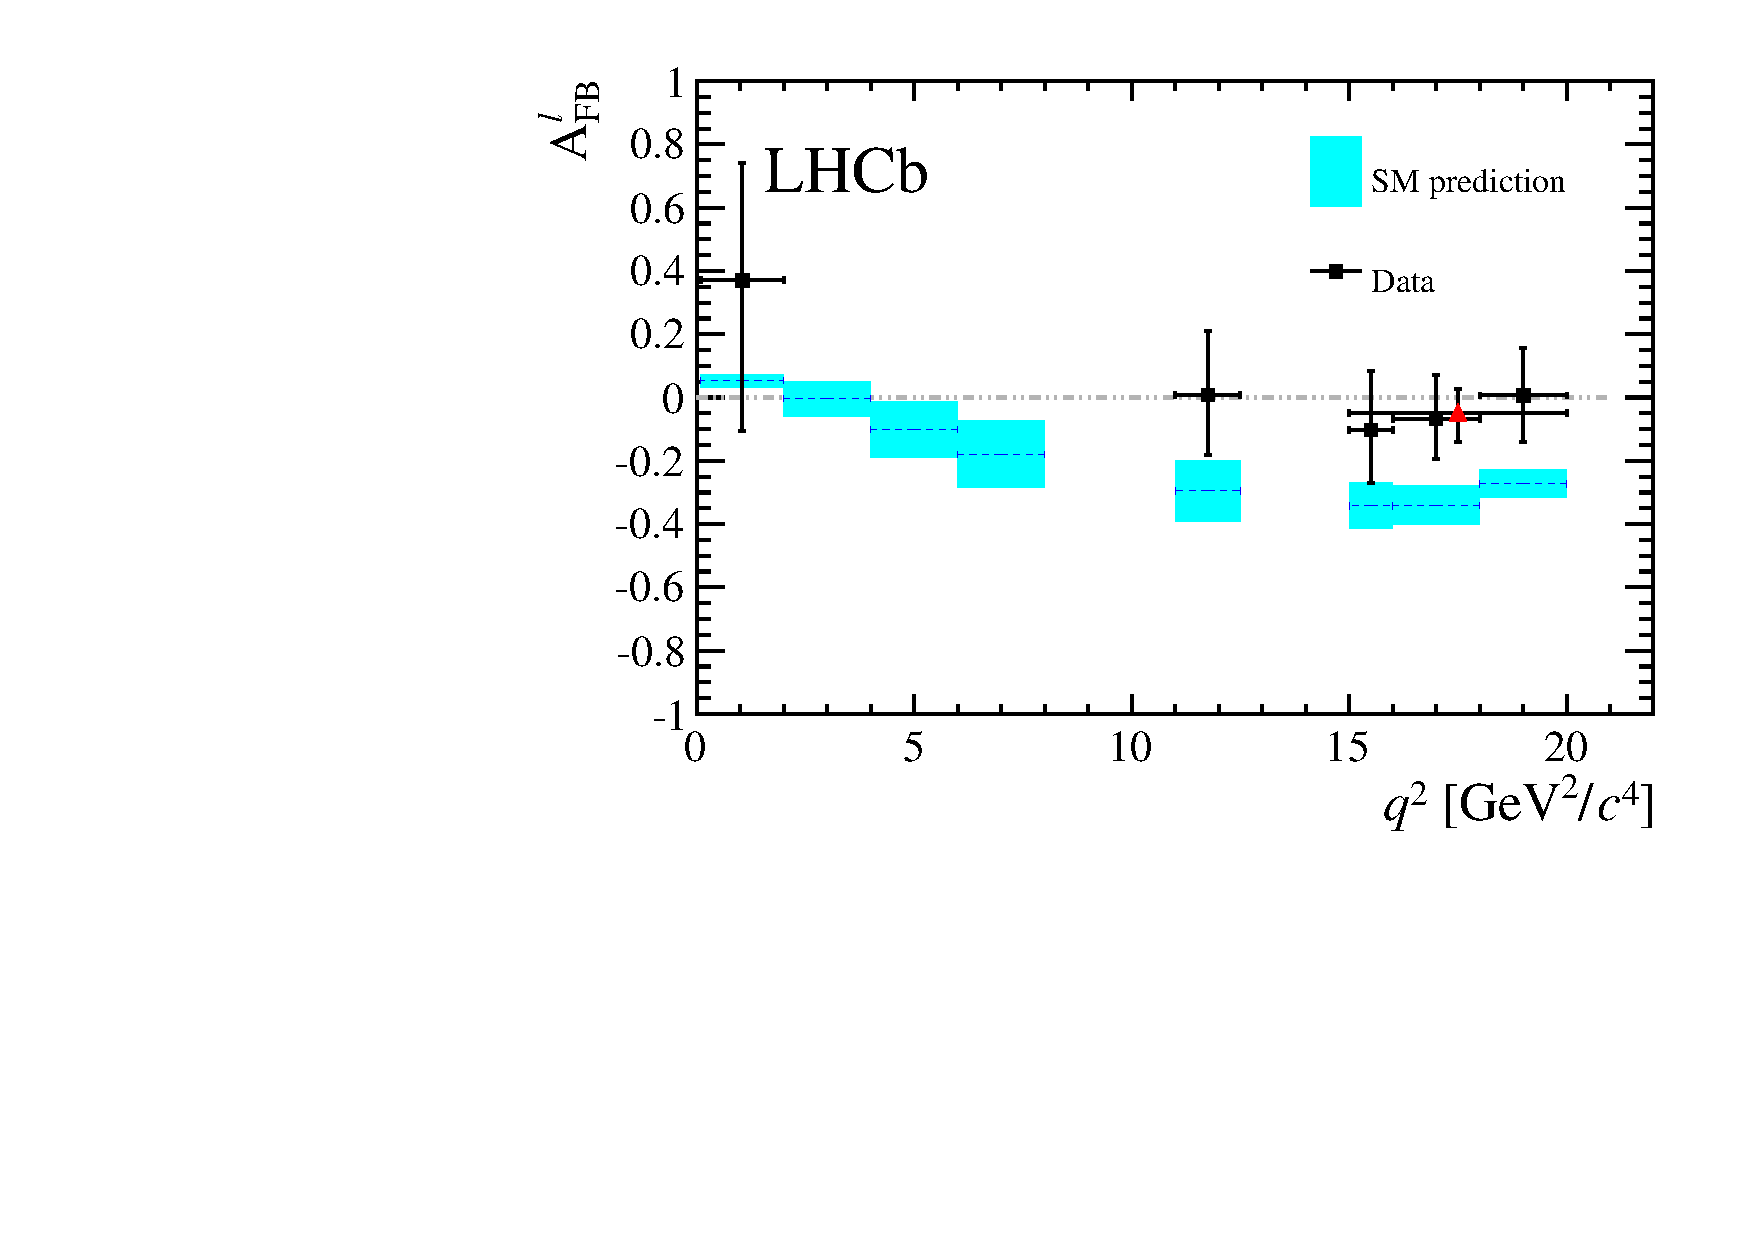
\includegraphics[width=0.8\textwidth]{Lmumu/figs/paper/figure8a.pdf}
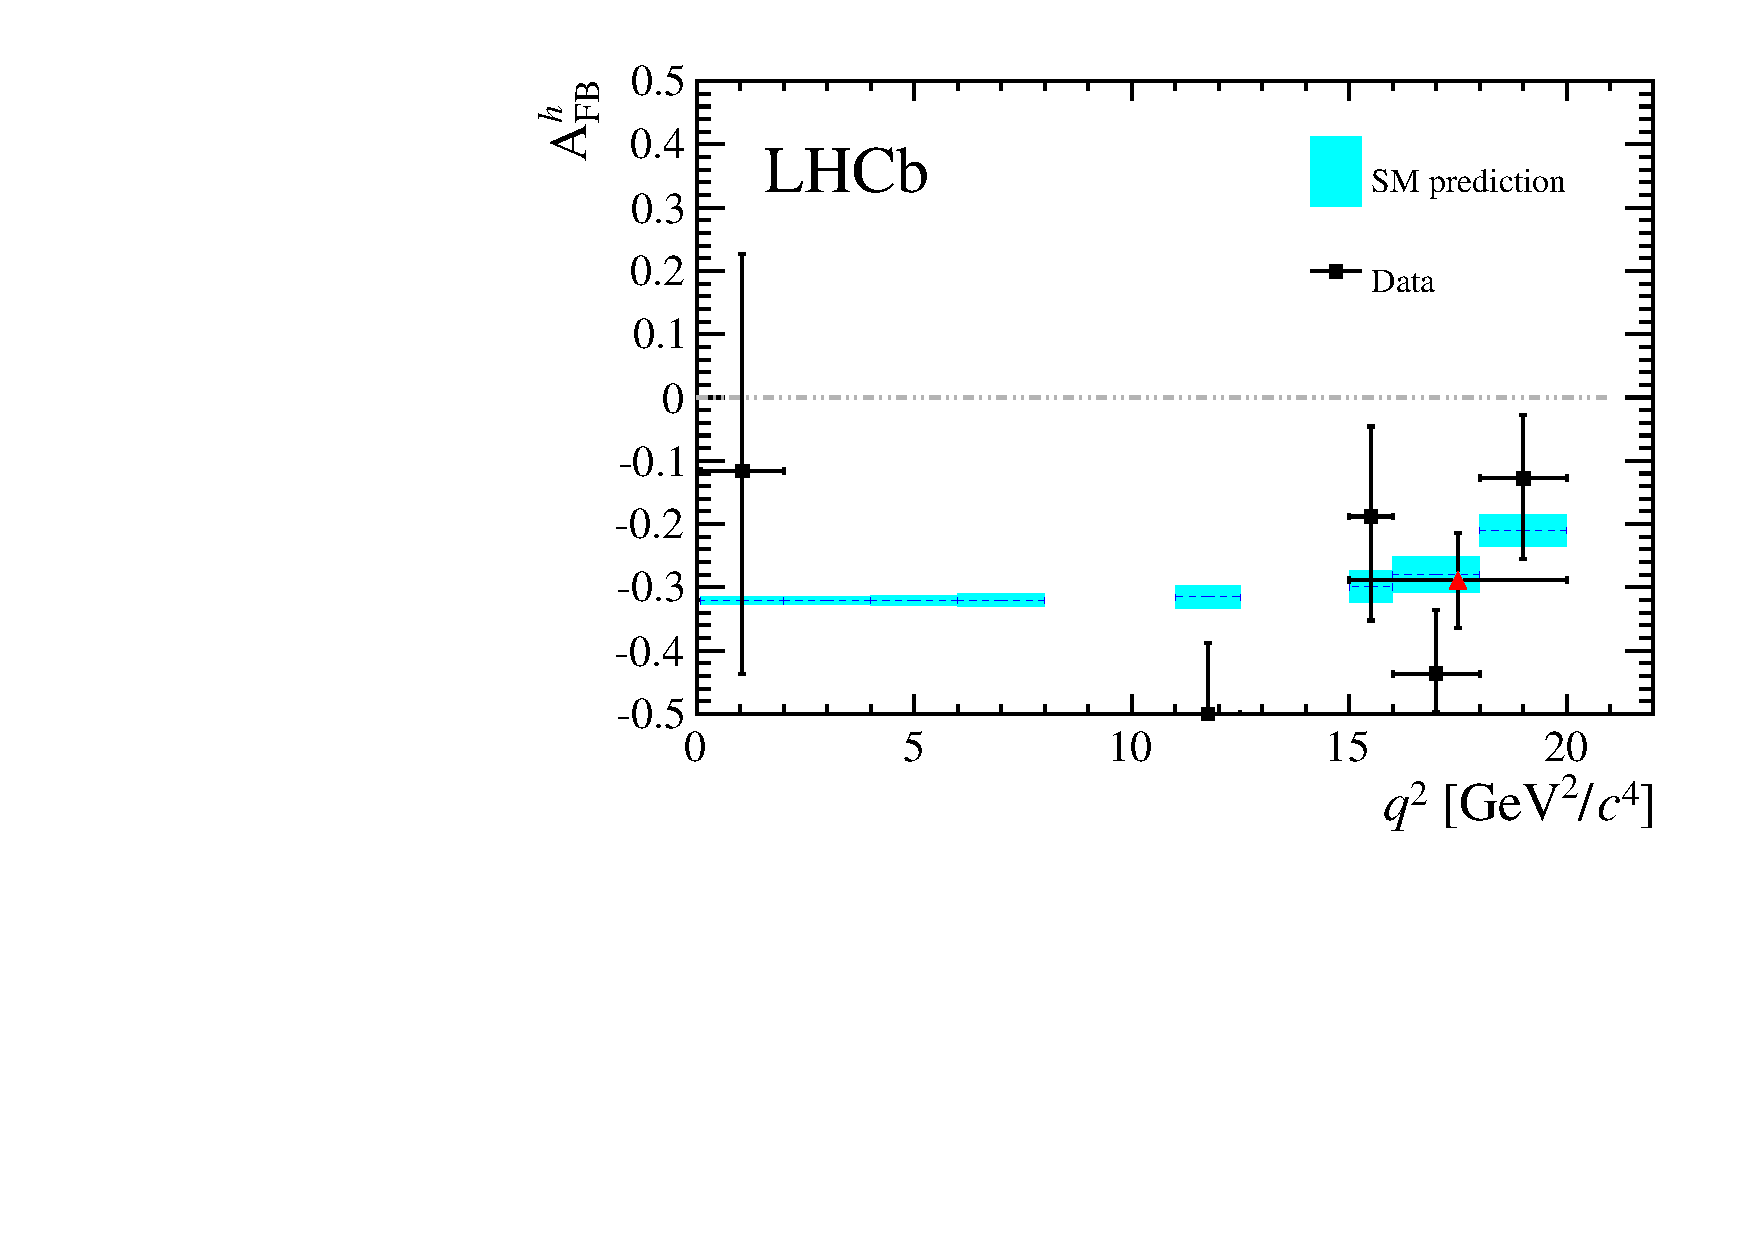
\includegraphics[width=0.8\textwidth]{Lmumu/figs/paper/figure8b.pdf}
\caption{Measured values of the leptonic (top) and the hadronic (bottom)
  forward-backward asymmetries. Data points are only shown for \qsq intervals 
  where the signal yield is found to be statistically significant, see text for details.
  The (red) triangle represents the values for the $15 < \qsq < 20$~\gevgevcccc
  integrated interval. Standard Model predictions are obtained from Ref.~\cite{Meinel:2014wua}.}
\label{fig:Afb_results}
\end{figure}

\begin{figure}[h]
\centering
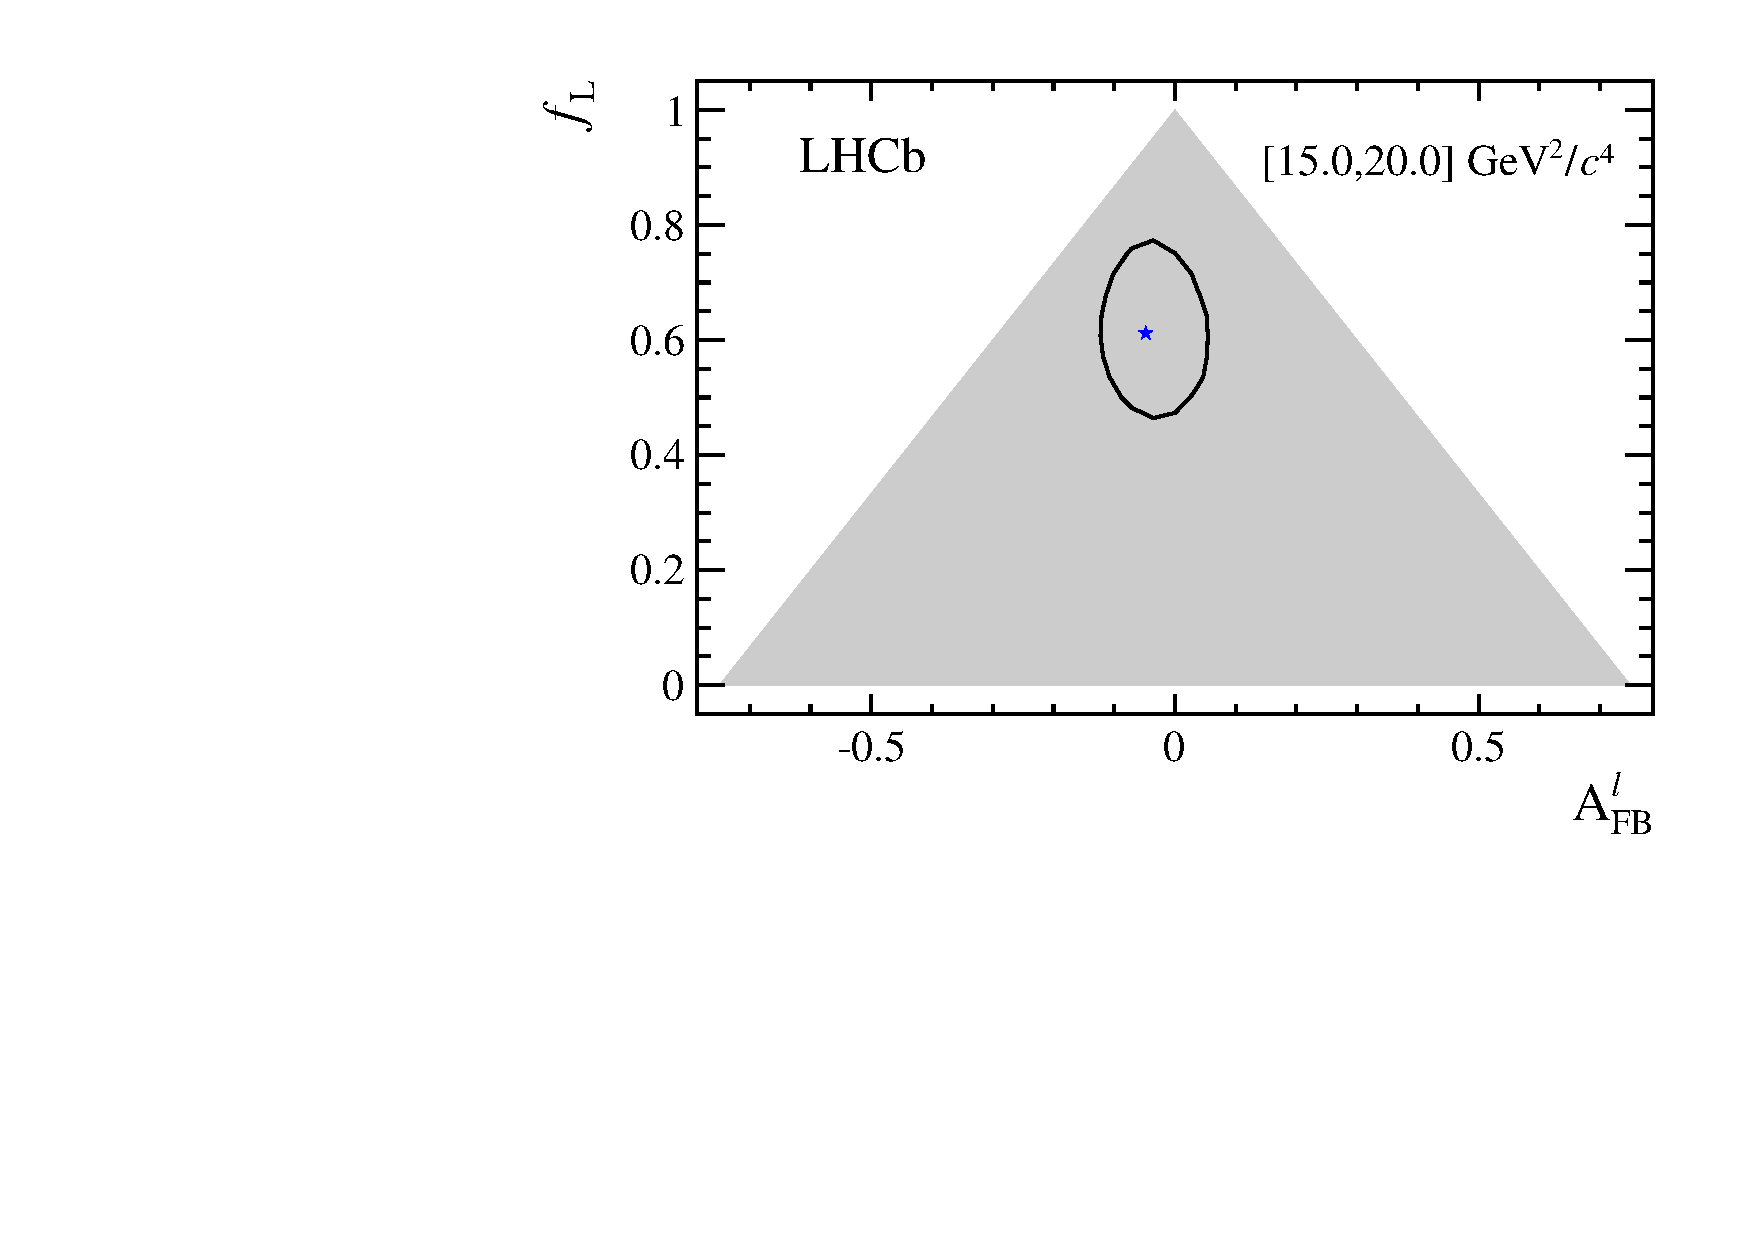
\includegraphics[width=0.49\textwidth]{Lmumu/figs/paper/figure9.pdf}
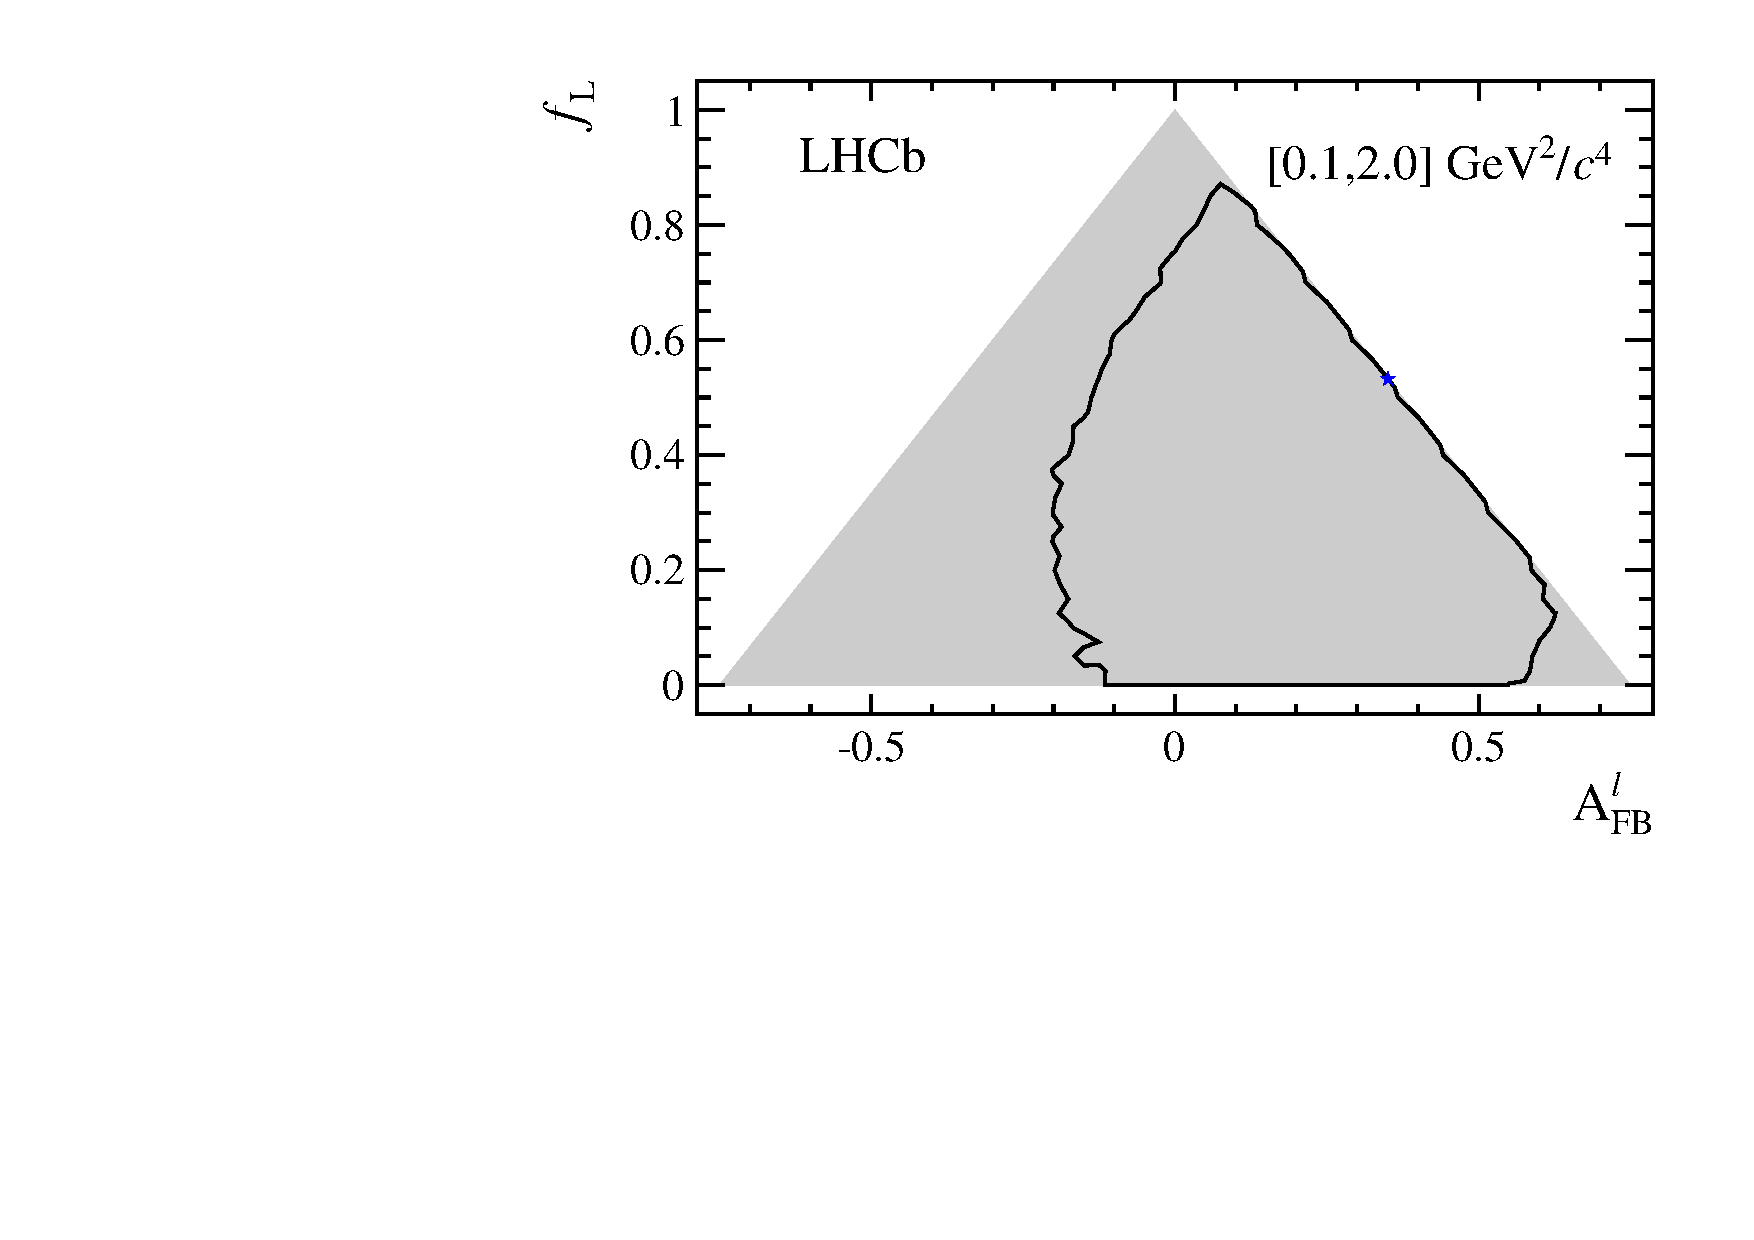
\includegraphics[width=0.49\textwidth]{Lmumu/figs/paper/figure10a.pdf}
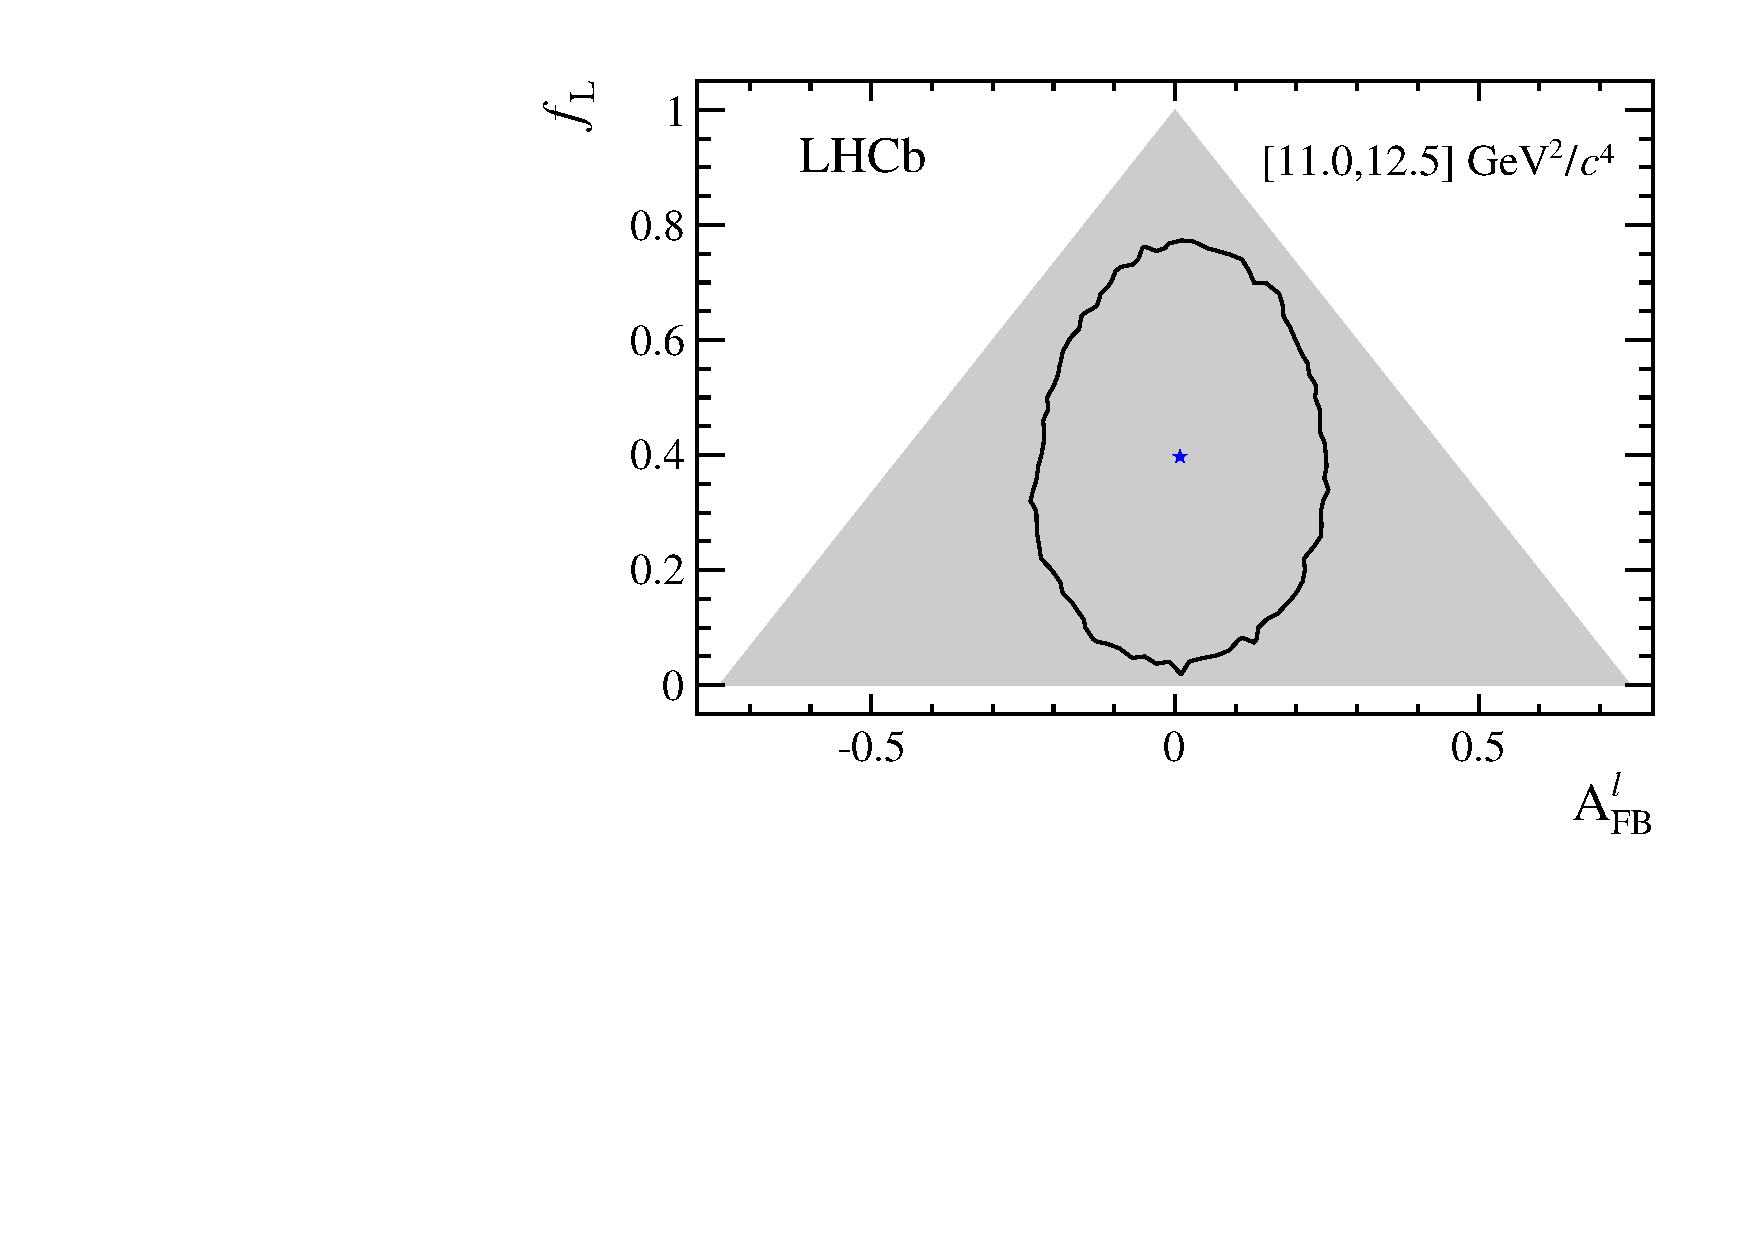
\includegraphics[width=0.49\textwidth]{Lmumu/figs/paper/figure10b.pdf}
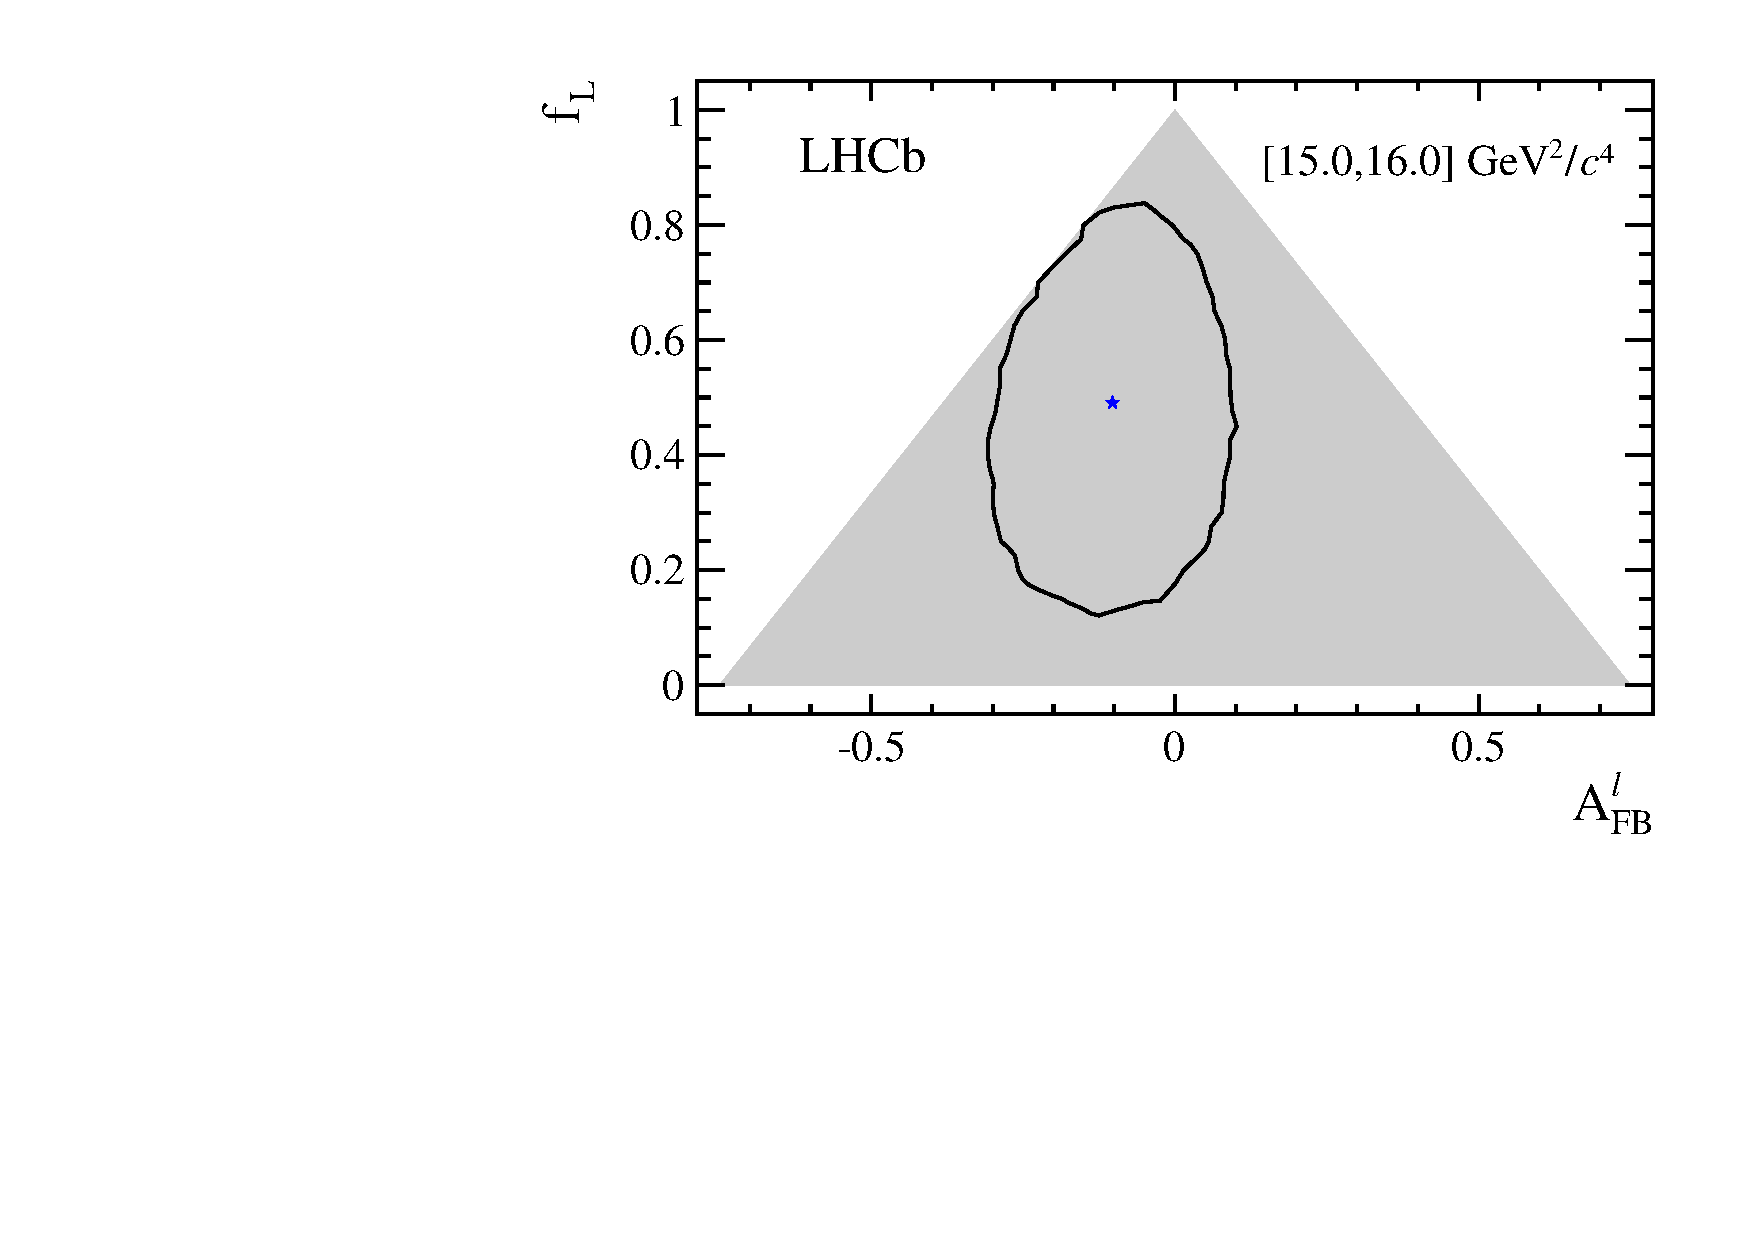
\includegraphics[width=0.49\textwidth]{Lmumu/figs/paper/figure10c.pdf}
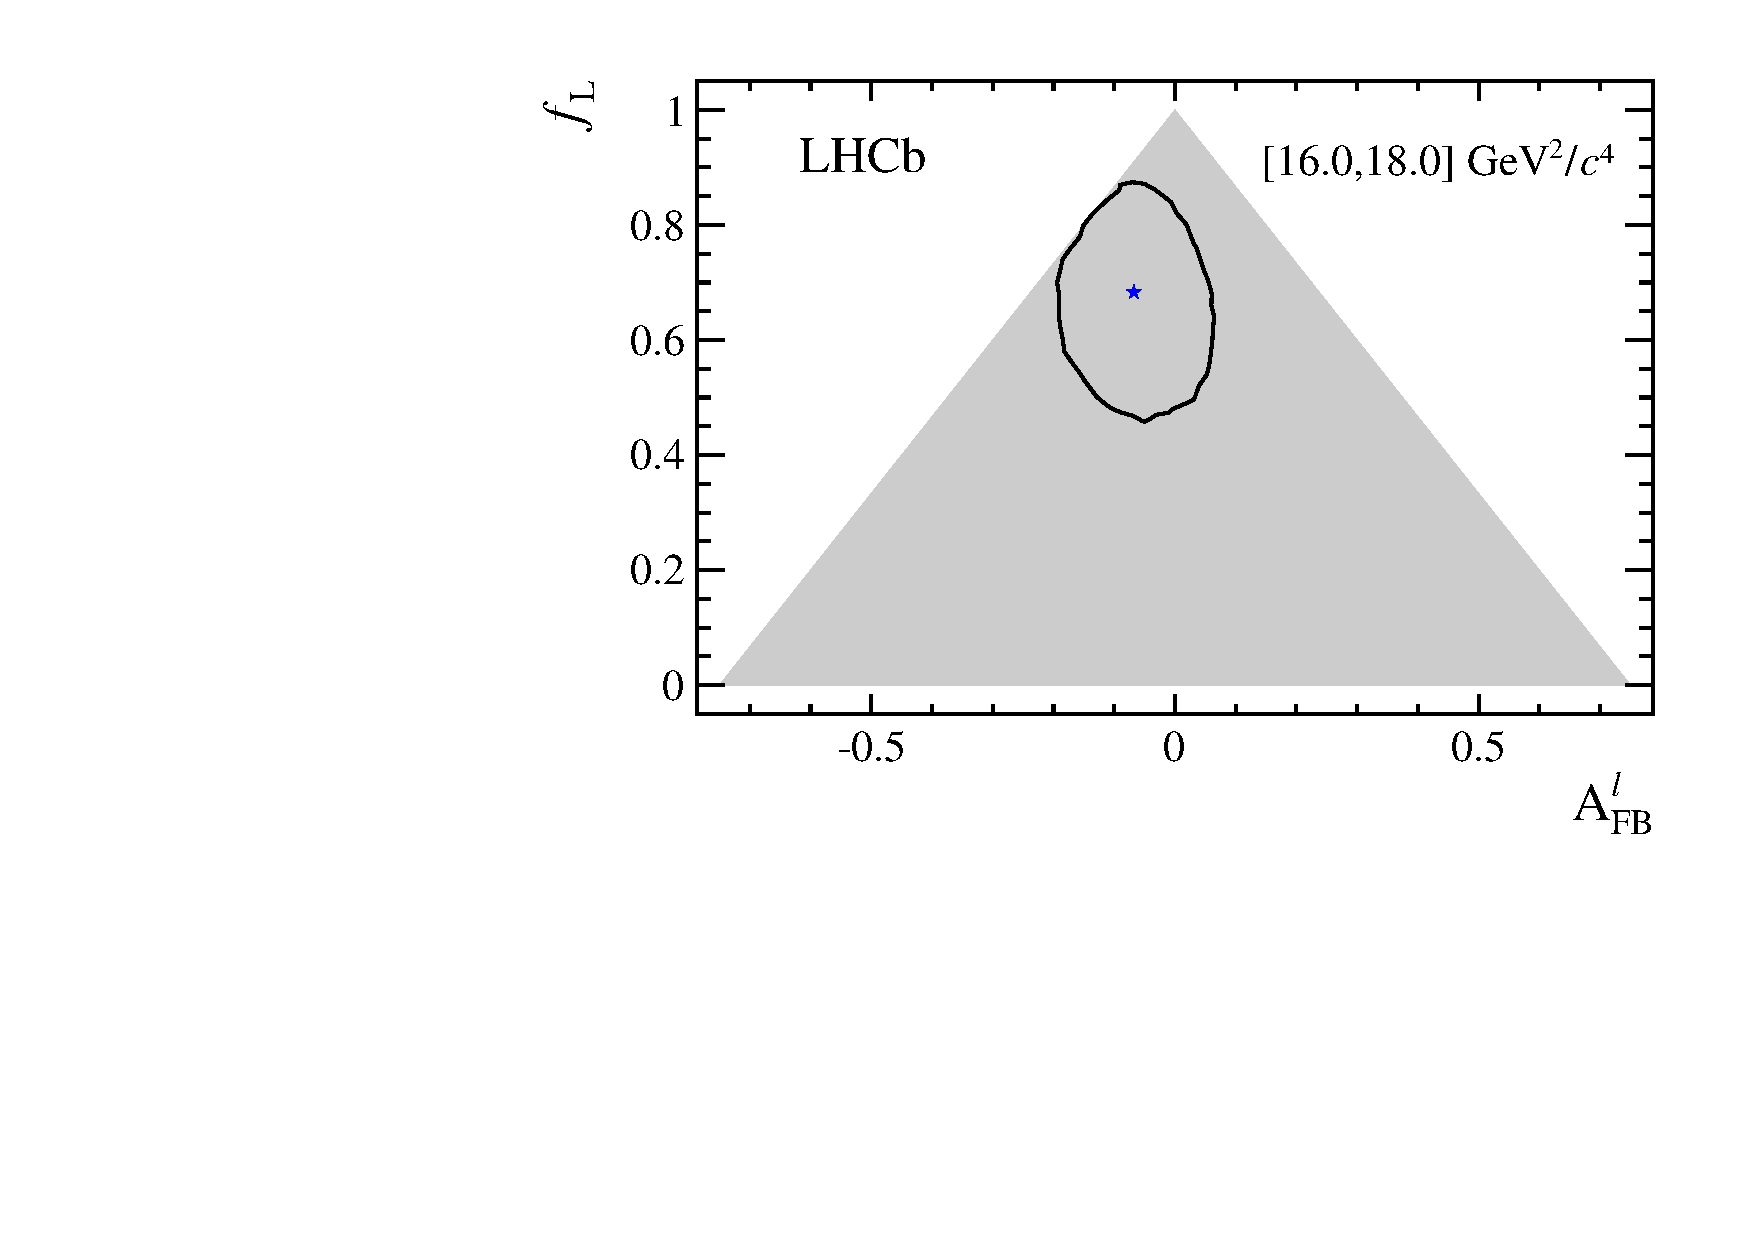
\includegraphics[width=0.49\textwidth]{Lmumu/figs/paper/figure10d.pdf}
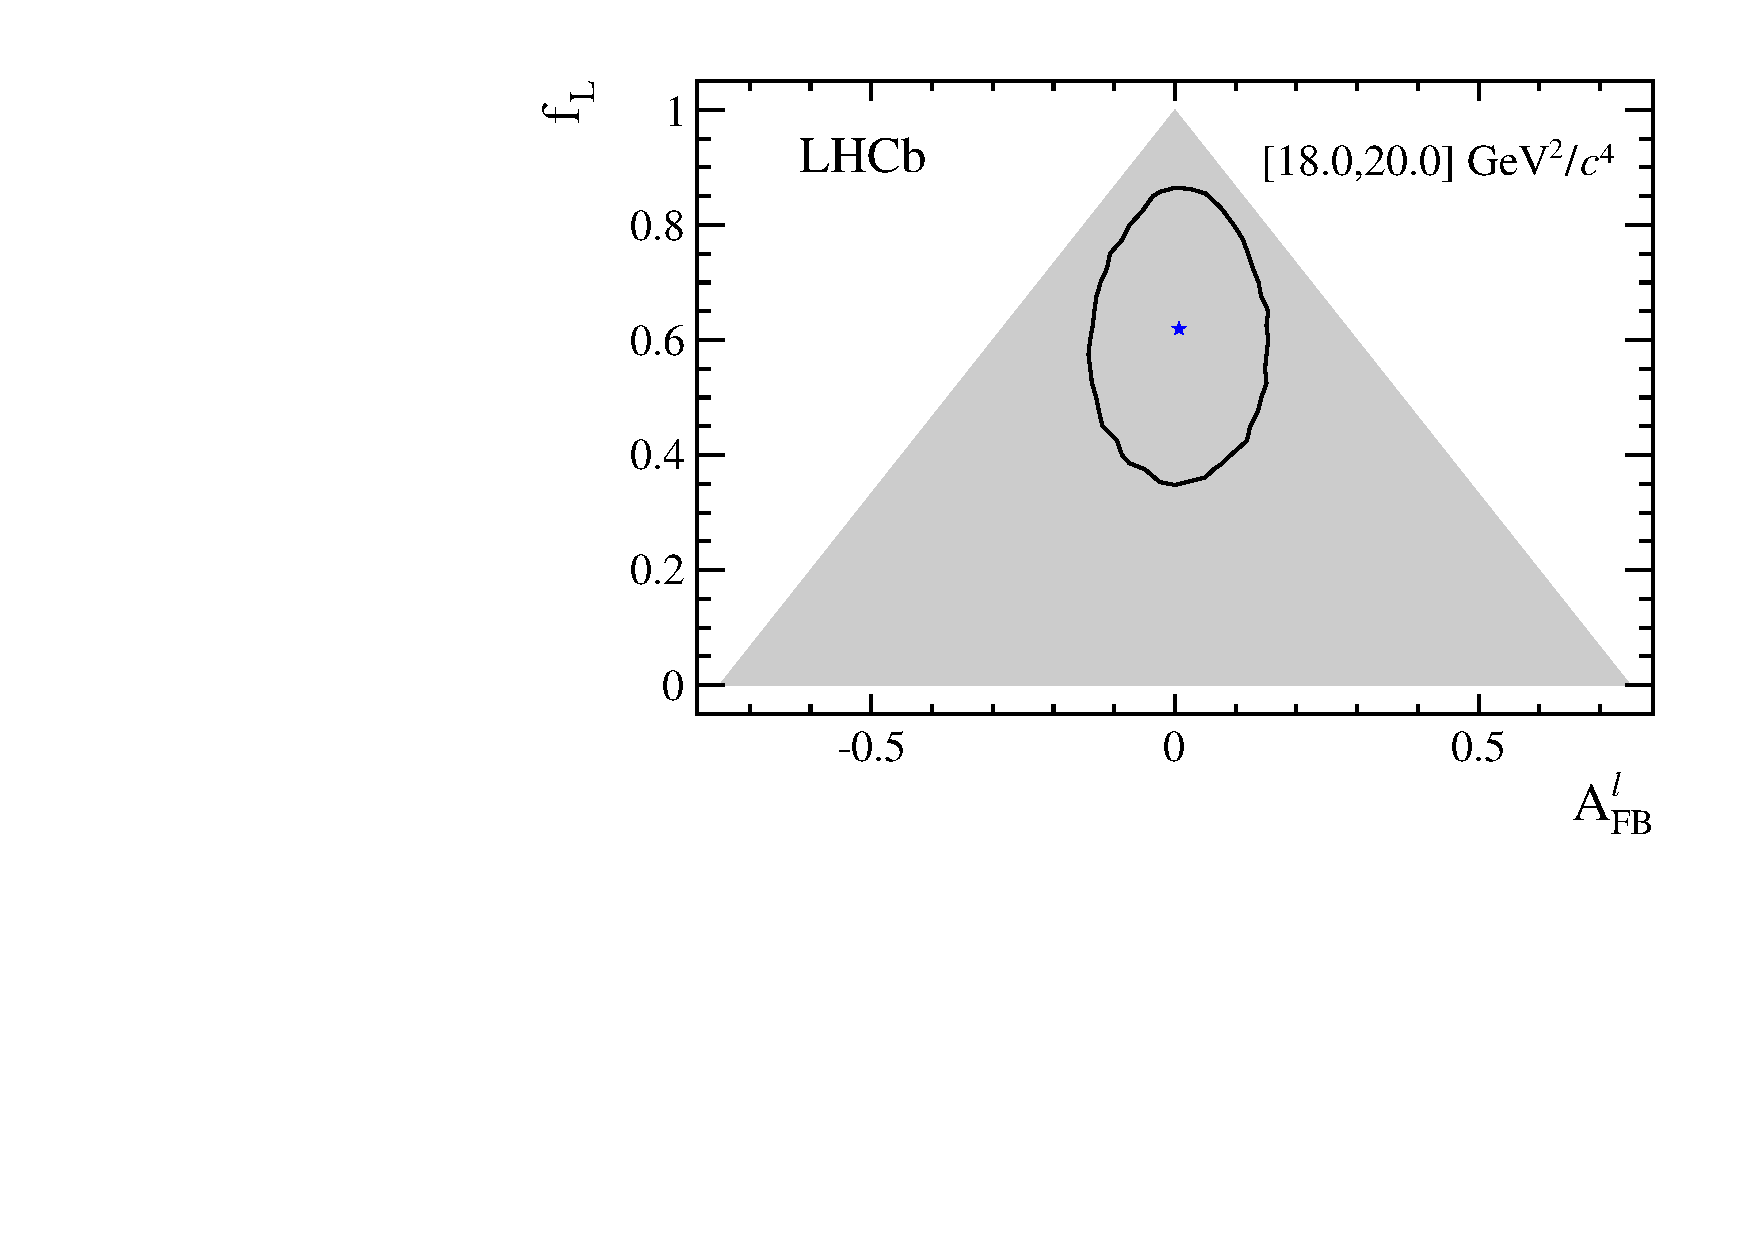
\includegraphics[width=0.49\textwidth]{Lmumu/figs/paper/figure10e.pdf}
\caption{Two-dimensional 68\,\% CL regions (black) as a
  function of $\afbl$ and $\fl$.  The shaded areas
  highlight the region in which the PDF is positive over the whole 
  $\cos \theta_{\ell}$ range. The best fit points are indicated by the (blue) stars. }
\label{fig:contours}
\end{figure}
